\section{Motivation and Challenges}
\label{sec:dataset-analysis}

\subsection{Inter-layer deduplication} Although Docker uses copy-on-write file
system to minimize redundant data inside each image and supports the sharing of
layers among different images to remove redundant data in the Docker registry
backend storage system, a large amount of duplicated files are observed among
layers within different images.
%
According to the deduplication analysis on Docker Hub
dataset~\cite{dedupanalysis}, only 3.2\% of files are unique, resulting in
deduplication ratio of 2x in terms of capacity.
%
\footnote{Deduplication ratio is only 2x despite the 97\% of redundant data
because most of the unique files are huge in szie.} 
%
These large amount of duplicated files shared among different layers associated
with different images are mainly executables, object codes, libraries, and
source codes, probably imported by different image developers using the same
package installers or version control systems such as \texttt{apt},
\texttt{pip} or \texttt{git} to install or get similar dependencies or source
codes.  

The current layer-level content addressable storage system design can not
provide \texttt{file-level deduplication} among different layers.
%
As containerization frameworks like Docker and Kubernetes keep gaining
popularity, more applications are encapsulated into images, pushed into
registry, and stored on Cloud.
%
Furthermore, due to \emph{R}-way replication, the amount of layers data grows
exponentially and will explode in future.
%
This large volume data management challenge can not be solved by just adding
more disks and goes beyond just hardware upgrade or even datacenter expansion.
%such as missive and slow data migration during scale-out or scale-up.
 
File-level deduplication can help solve this challenge by first decompressing
the compressed layer tarballs and then removing the duplicate files across
different layers.
%
This way layer dataset stored on registry can be largely reduced for better
data management.
%
However, to \texttt{GET} a layer from a registry which employs file-level
deduplication requires restoring a layer, which involves fetching the files,
layer archiving, and layer compression.
%
These extra operations incur a considerable overhead. \footnote{\texttt{GET}
layer time is crucial as it comprises ??\% of the container startup time.}
%
In this paper, we explore if it is possible to deduplicate layers without
sacrificing the \texttt{GET} layer performance.
%   
%Consider that deduplication incurs a performance overhead and the current
%Docker registry already stores layers in compressed format to save space and
%network transfer overhead. We first analyze the space efficiency of a registry
%that performs decompression and file-level deduplication and compare it to a
%registry that naively stores compressed layers.

%In Figure~\ref{fig:cacheefficiency}, the x-axis values correspond to the sizes
%of $5$ samples of registry data of varying sizes with traditional layer
%compression. For a traditional registry, the compressed layer tarballs will be
%kept as is.  While a registry with file-level deduplication will store
%\emph{deduplicated} layers (i.e., unique files).  The y-axis shows how much
%space a registry with file-level deduplication can save over compressed layer
%tarballs.  For the first two samples of the dataset, with size less than
%$20$~GB, there is no benefit to \emph{deduplicate} layers because the
%deduplication ratio is very low.  However, when the dataset size is $200$~GB
%and over, we can save over $40\%$ more space increasing almost linearly with
%the size of the layer dataset.  This verifies the benefit of deduplicating
%layers as the registry size increases.  Before describing Sift, we must
%understand the storage pressure and trends in the access patterns of the
%Docker registries at the layer and repository level.

\subsection{Predictable User Access}
%
%\begin{figure*}[t]
%		\begin{minipage}{0.32\linewidth}
%			\centering
%			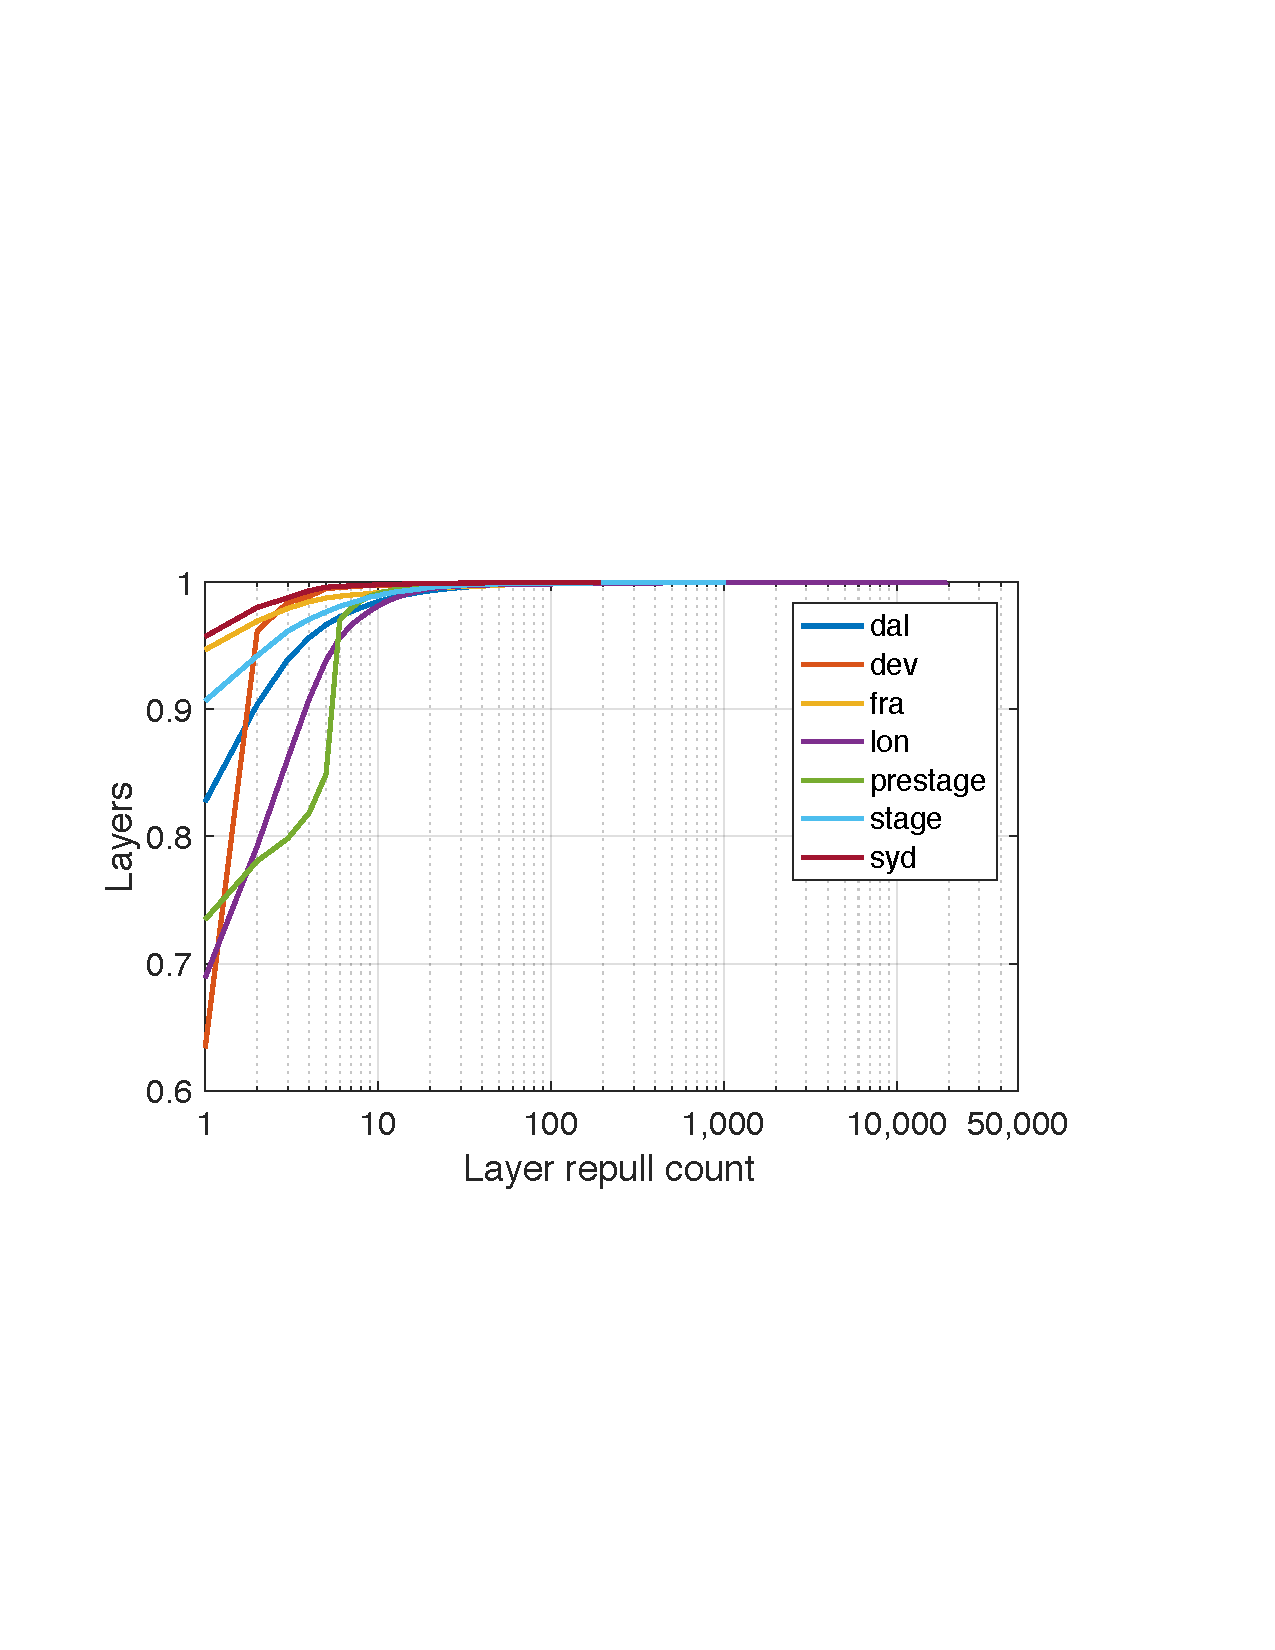
\includegraphics[width=1\textwidth]{graphs/cdf-layer-repull-by-same-client.pdf}
%			%\caption{CDF of layer repull count.}
%		%	\vspace{-3pt}
%			\label{fig:layer-repull-cdf}
%		\end{minipage}
%			\begin{minipage}{0.32\linewidth}
%				\centering
%				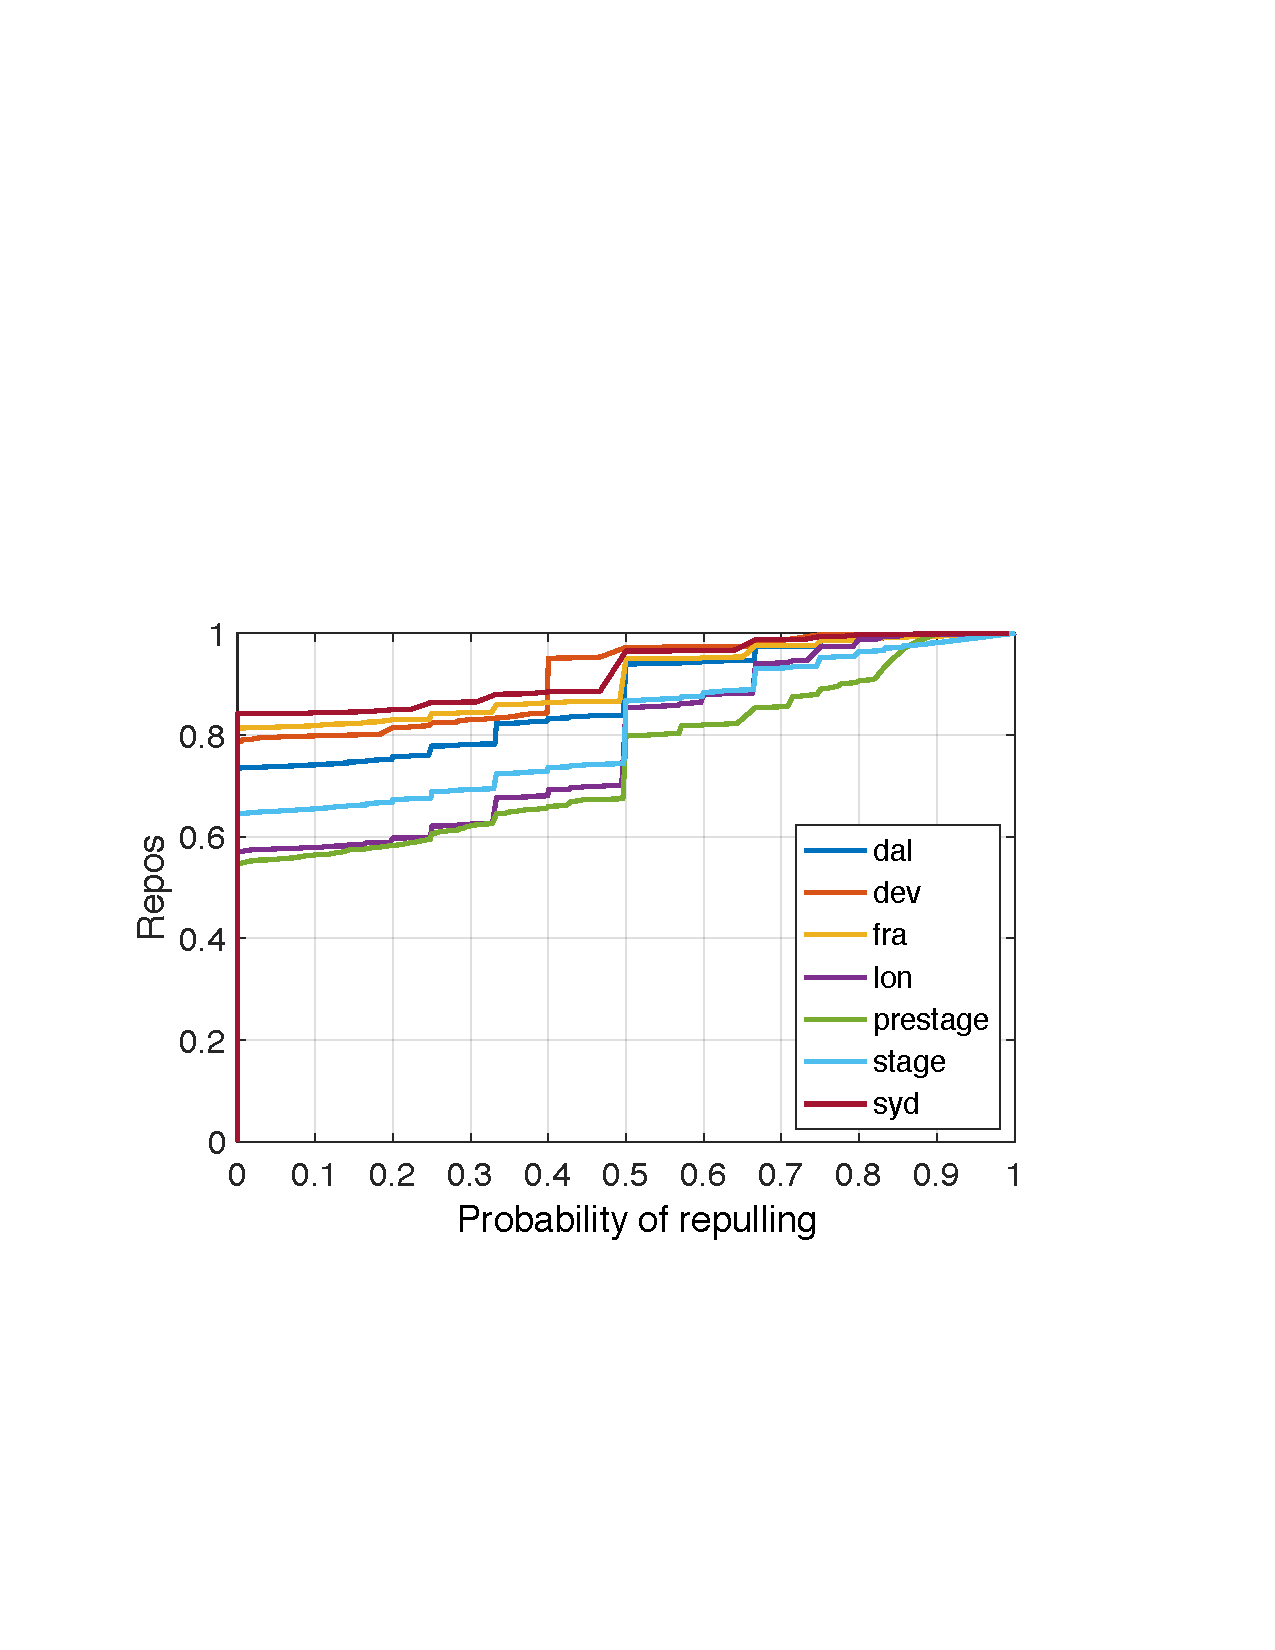
\includegraphics[width=1\textwidth]{graphs/cdf-repo-repull-ratio-by-same-client.pdf}
%				%\caption{PDF of repository repulling probability.}
%				%	\vspace{-3pt}
%				\label{fig:repo-repull-cdf}
%			\end{minipage}
%		\begin{minipage}{0.32\linewidth}
%			\centering
%			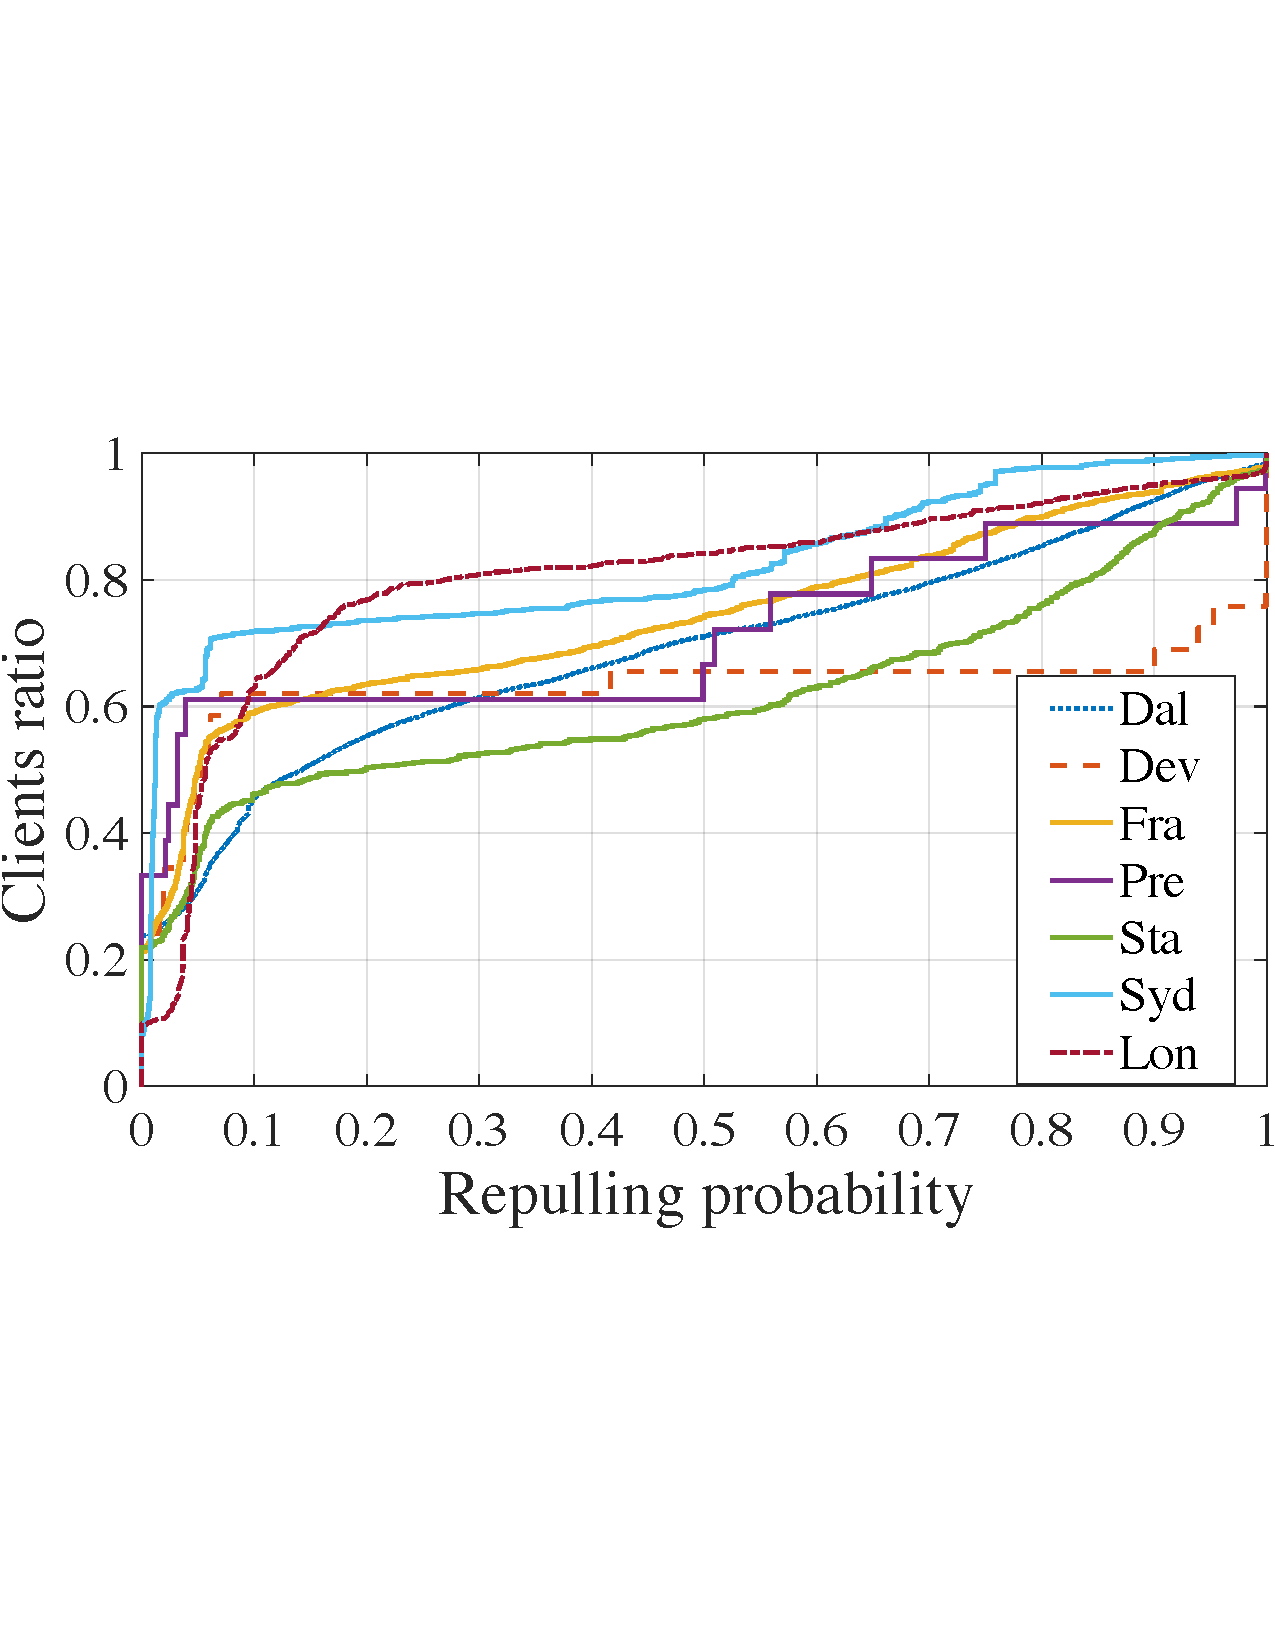
\includegraphics[width=1\textwidth]{graphs/cdf-client-repull-layer-request-ratio.pdf}
%			%
%			%	\vspace{-3pt}
%			\label{fig:client-repull-cdf}
%		\end{minipage}
%	\caption{PDF of client repull count, repository repulling probability, and client repulling probability..}
%\end{figure*}

%\begin{figure}[!t]
%	\centering
%	\subfigure[\texttt{GET} layer request count]{
%		\includegraphics[width=0.22\textwidth]{graphs/cdf-layer-repull-ratio-by-same-client.pdf}
%		\label{fig:layer-repull-cdf}
%	}
%%	\subfigure[Repository repulling probability]{
%%		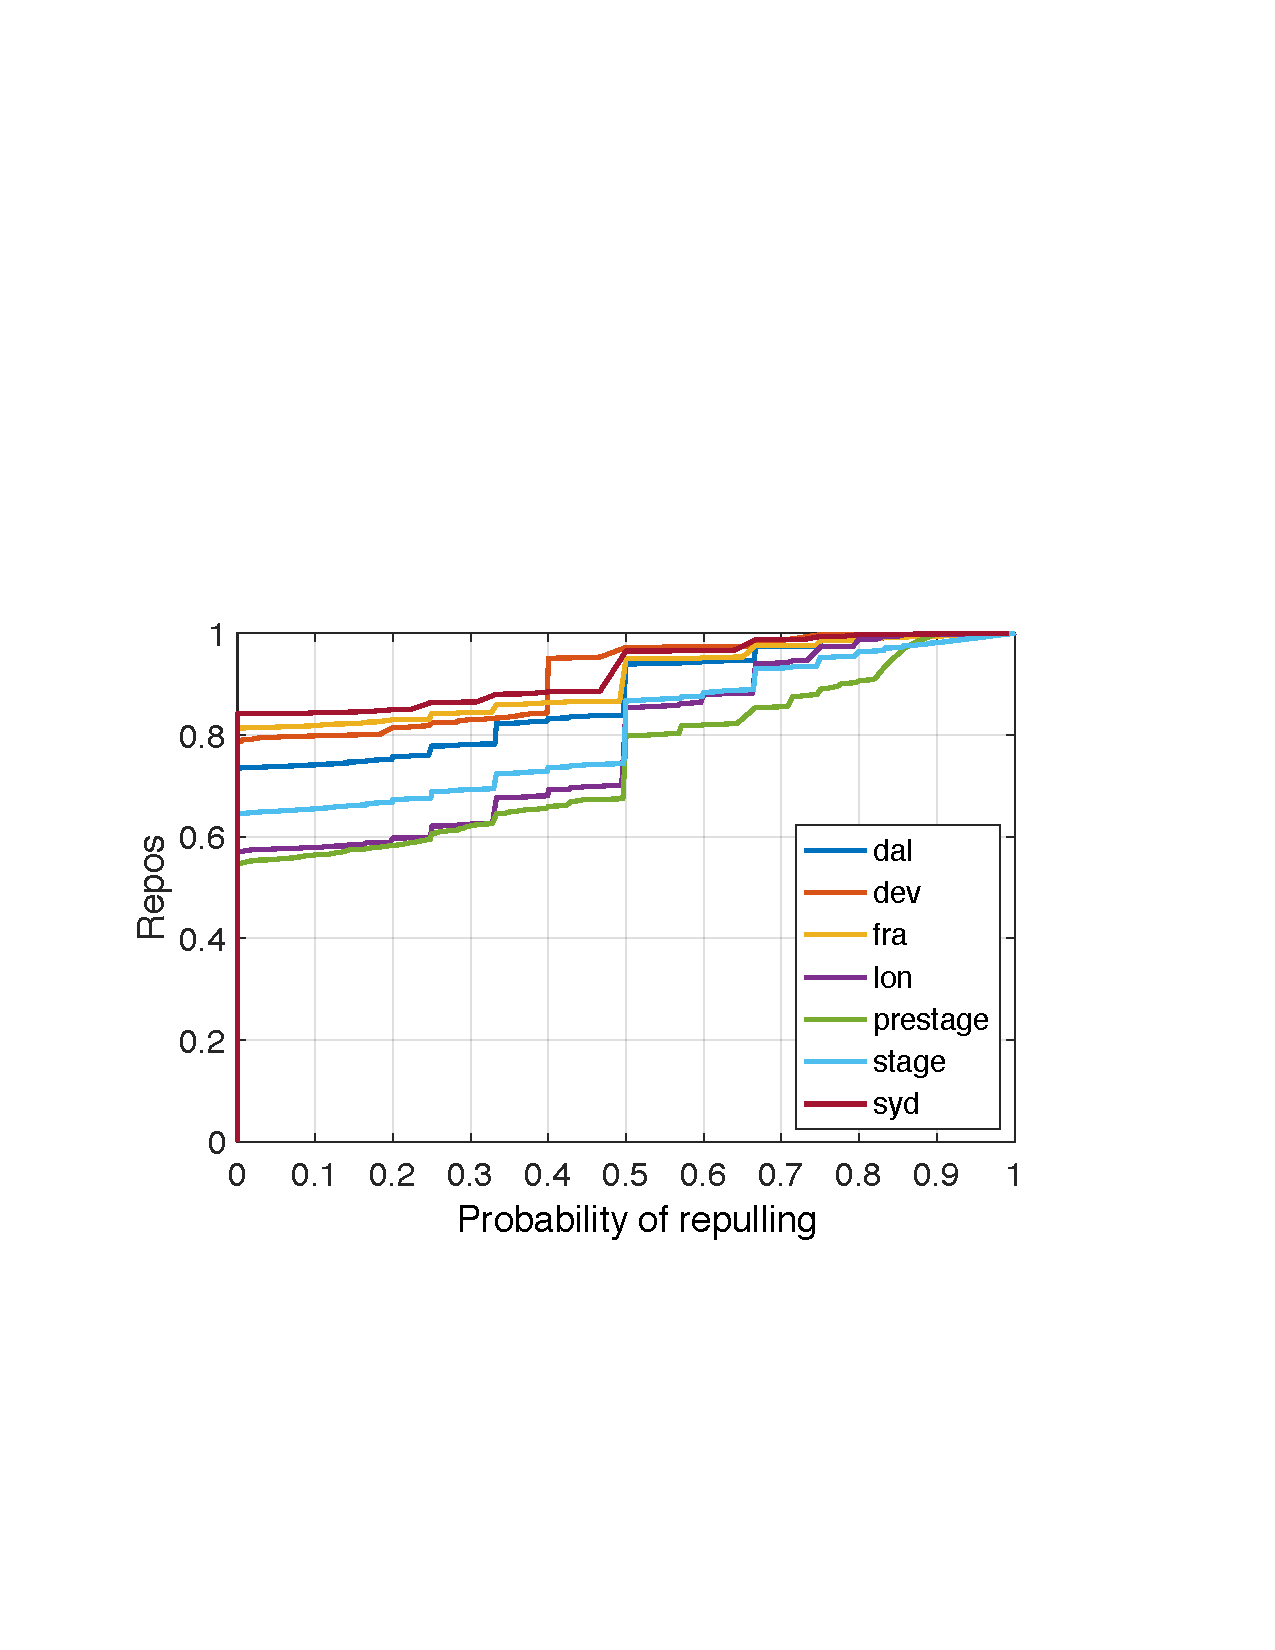
\includegraphics[width=0.2\linewidth]{graphs/cdf-repo-repull-ratio-by-same-client.pdf}
%%		\label{fig:repo-repull-cdf}
%%	}
%	\subfigure[Client repulling probability]{
%	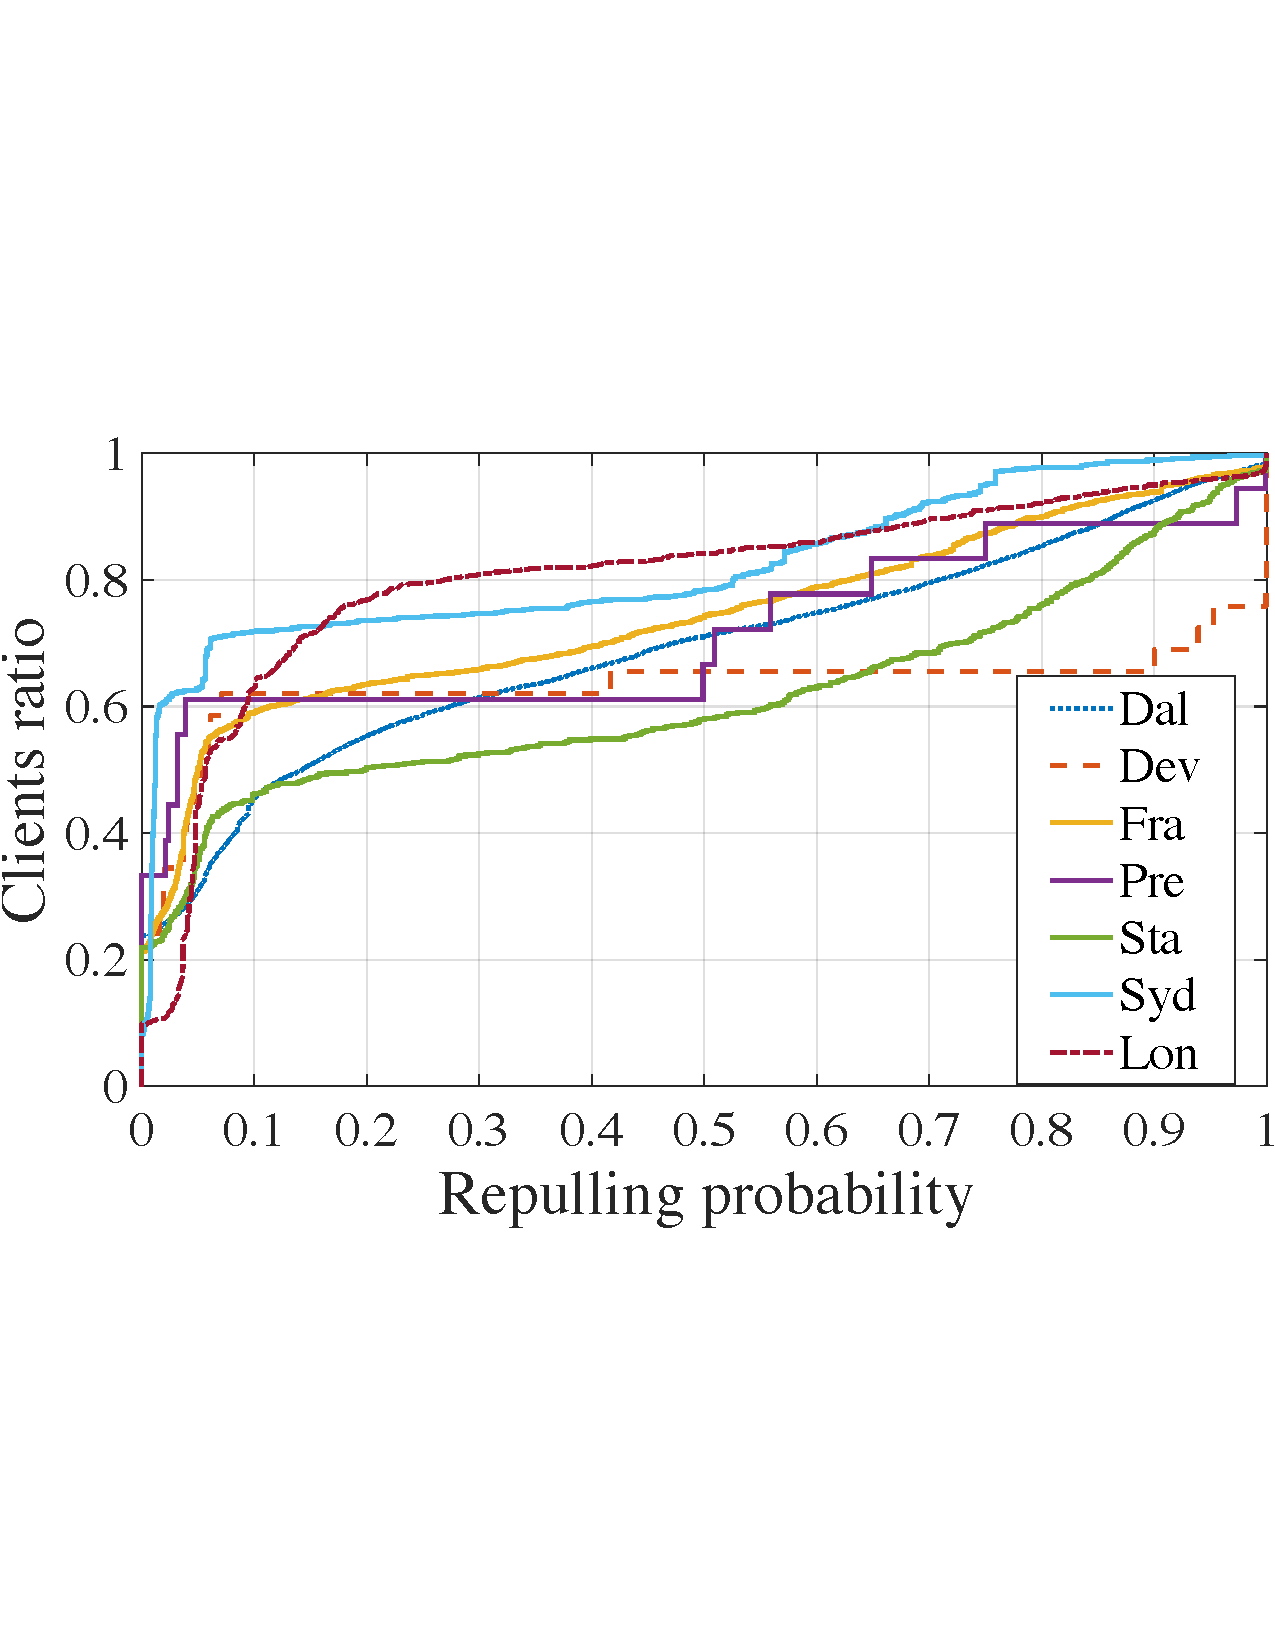
\includegraphics[width=0.2\textwidth]{graphs/cdf-client-repull-layer-request-ratio.pdf}
%   \label{fig:client-repull-cdf}
%}
%	\caption{CDF of \texttt{GET} layer request count and client repulling probability.}
%	\label{fig-repull}
%\end{figure}
%






\begin{figure*}[t]
        \centering
        \begin{minipage}{0.3\textwidth}
                \centering
                \includegraphics[width=0.9\textwidth]{{graphs/cdf-layer-repull-ratio-by-same-client.pdf}
                \caption{CDF of \texttt{GET} layer request count}
                \label{fig:layer-repull-cdf}
        \end{minipage}%
        \begin{minipage}{0.3\textwidth}
                \centering
                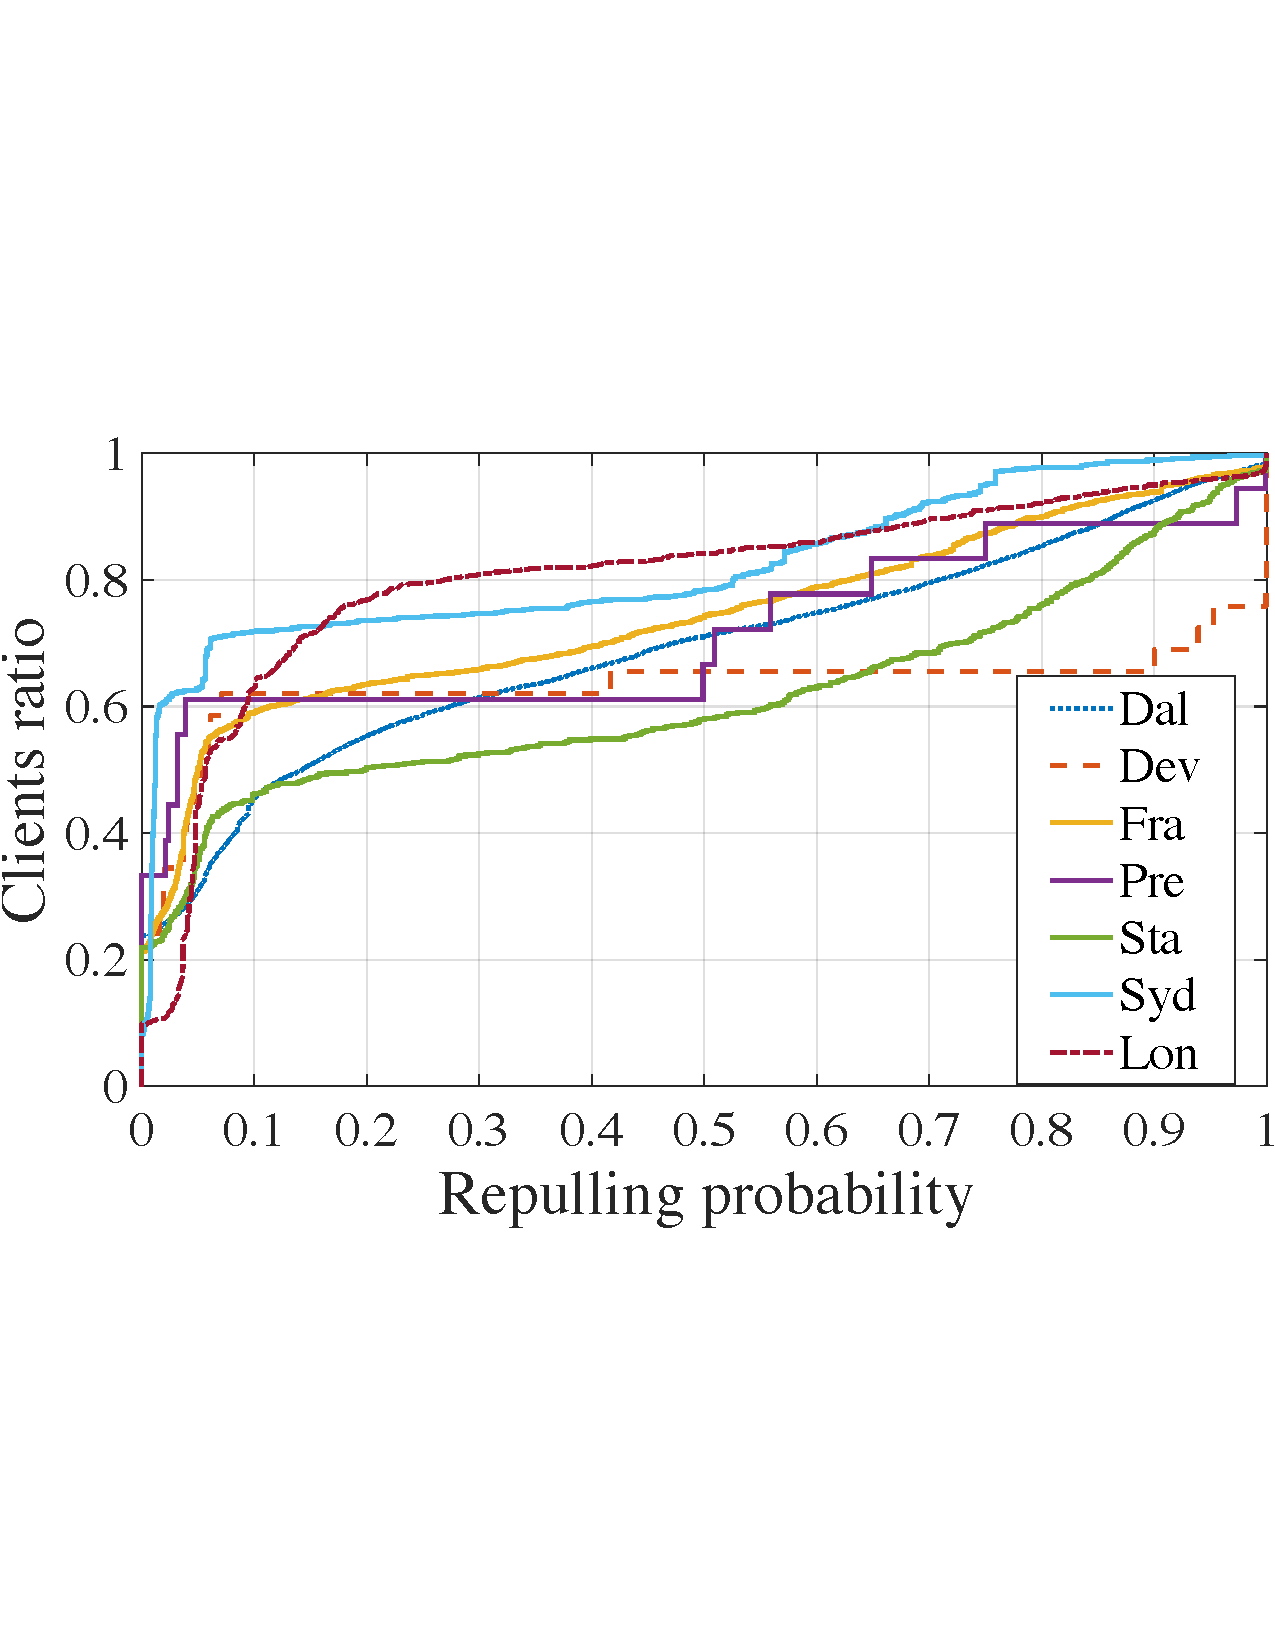
\includegraphics[width=0.9\textwidth]{graphs/cdf-client-repull-layer-request-ratio.pdf}
                \caption{CDF of Client repulling probability}% of LRU cache and preconstruct cache.}
                \label{fig:client-repull-cdf}
        \end{minipage}%
        \begin{minipage}{0.3\textwidth}
        \centering
        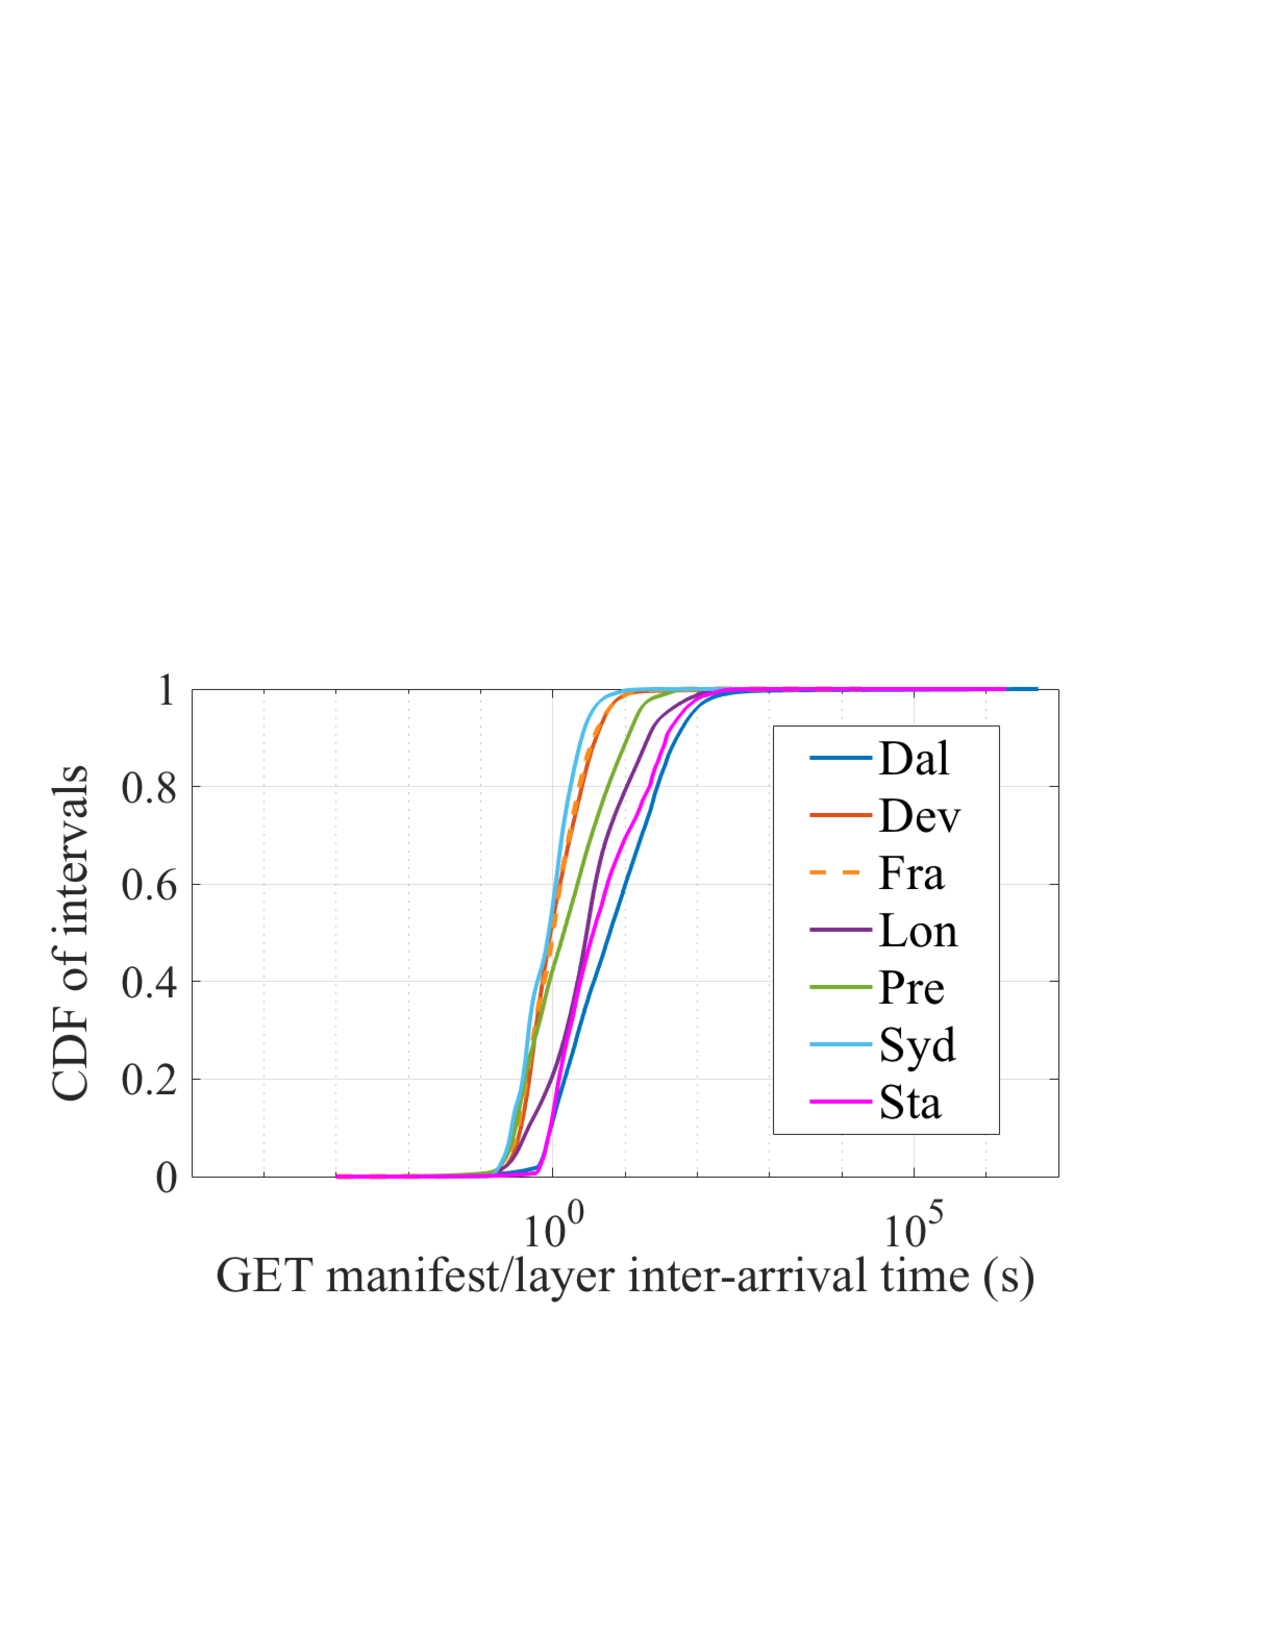
\includegraphics[width=0.9\textwidth]{graphs/GML-intervals.pdf}
        \caption{Intervals between \texttt{GET} manifest request and \texttt{GET} layer request}
        \label{fig:intervals}
   \end{minipage}
\end{figure*}





%\begin{figure}[!t]
%	\centering
%	\subfigure[CDF of compression ratio]{\label{fig_cdf_compression_ratio}
%		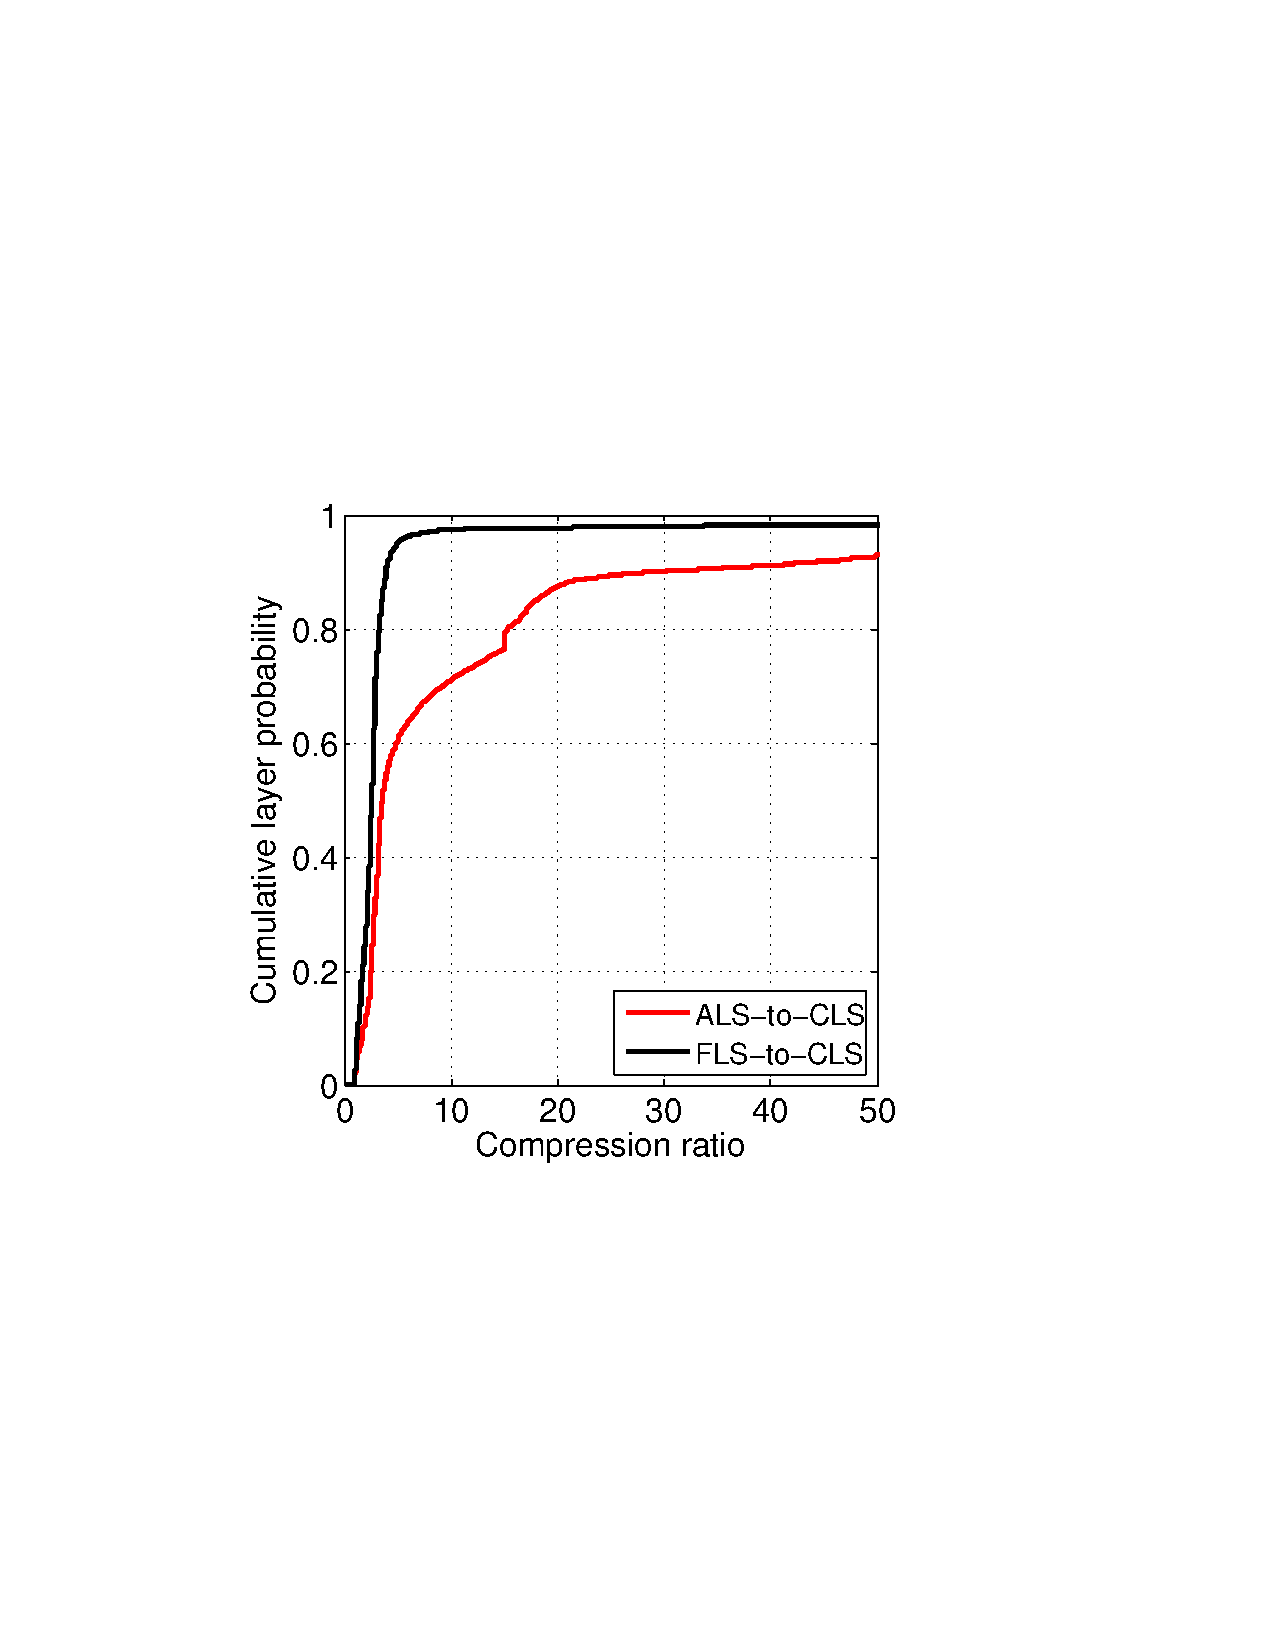
\includegraphics[width=0.23\textwidth]{graphs/cdf_compression_ratio.pdf}
%	}
%	\subfigure[Histogram of comp. ratios]{\label{fig_his_compression_ratio}
%		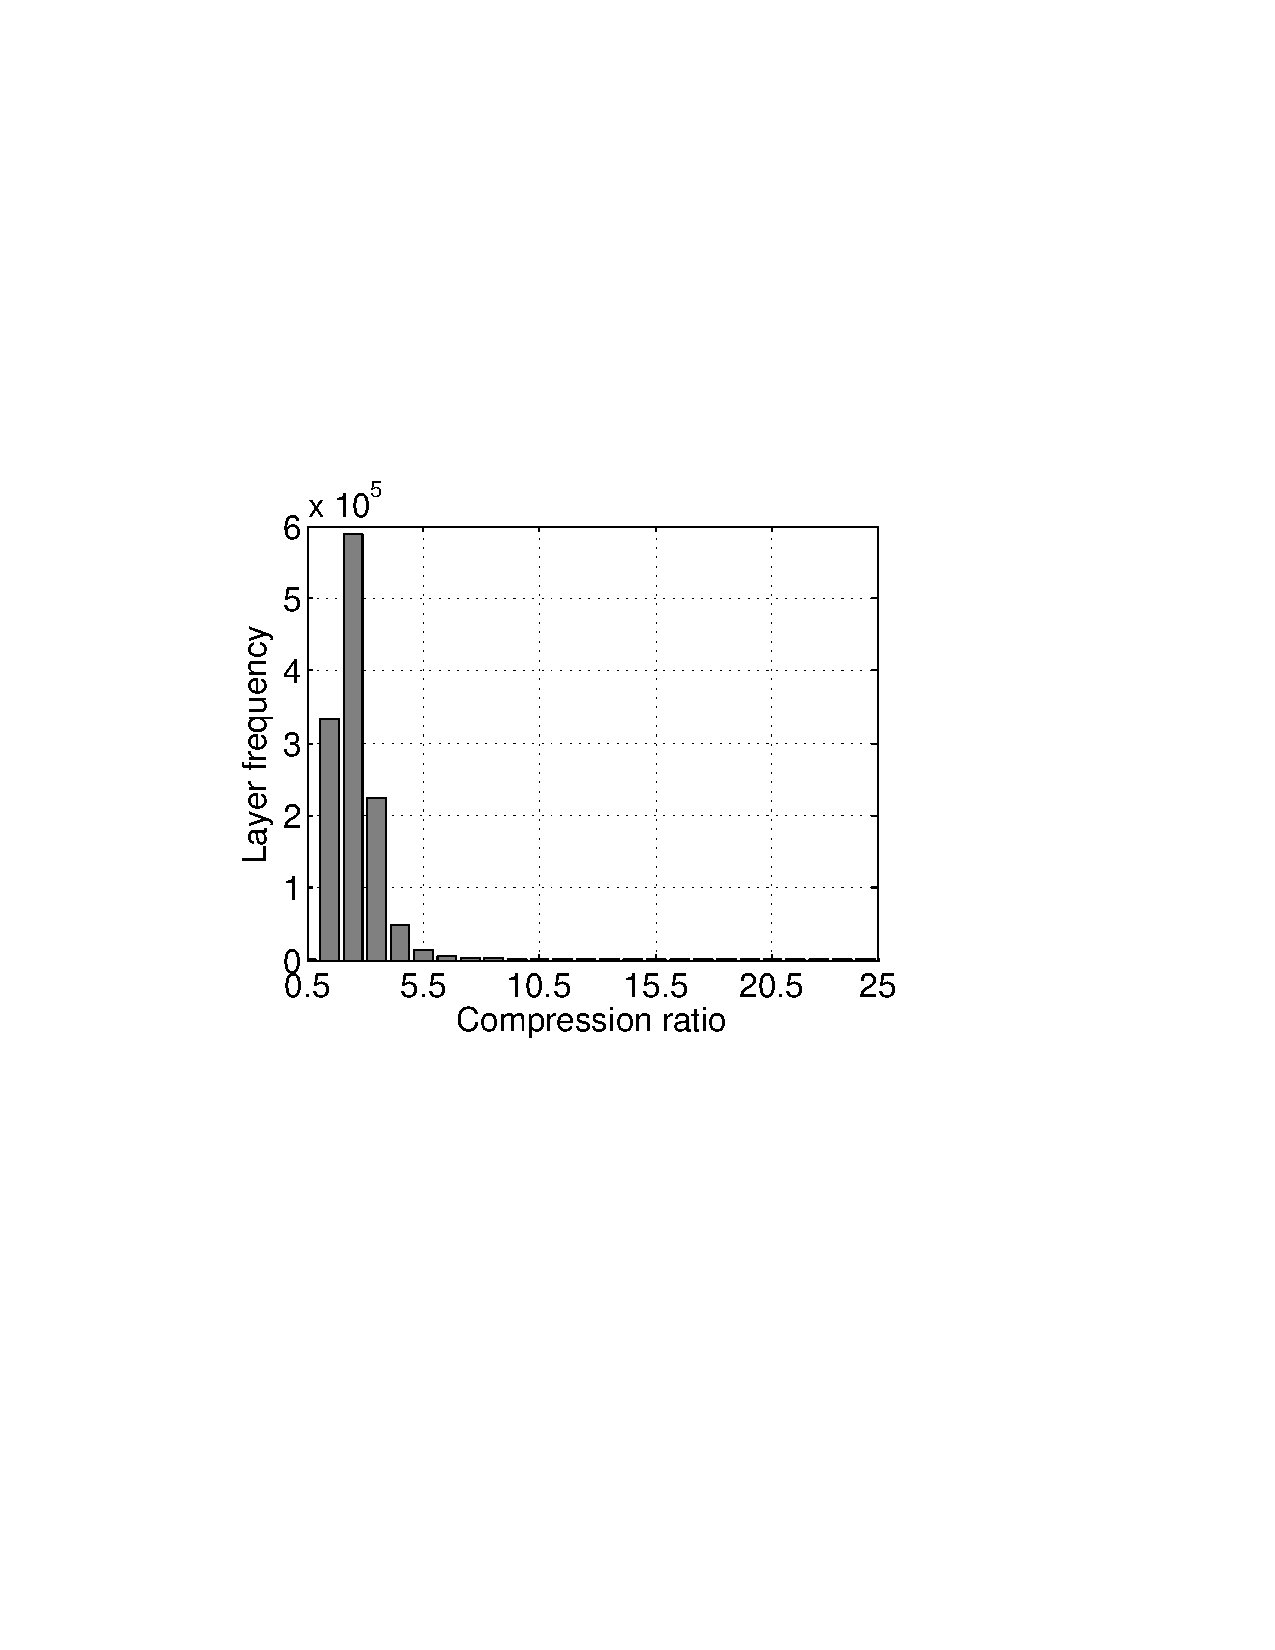
\includegraphics[width=0.223\textwidth]{graphs/his_compression_ratio.pdf}
%	}
%	\caption{Layer compression ratio distribution
%		%\vcomment{Different colors are used in figure (a) and (b) FLS/CLS\nancomment{will address later}}
%	}
%	\label{fig-compression-ratio}
%\end{figure}


%\begin{figure}[t]
%	\centering
%	\begin{minipage}{0.26\textwidth}
%		\centering
%		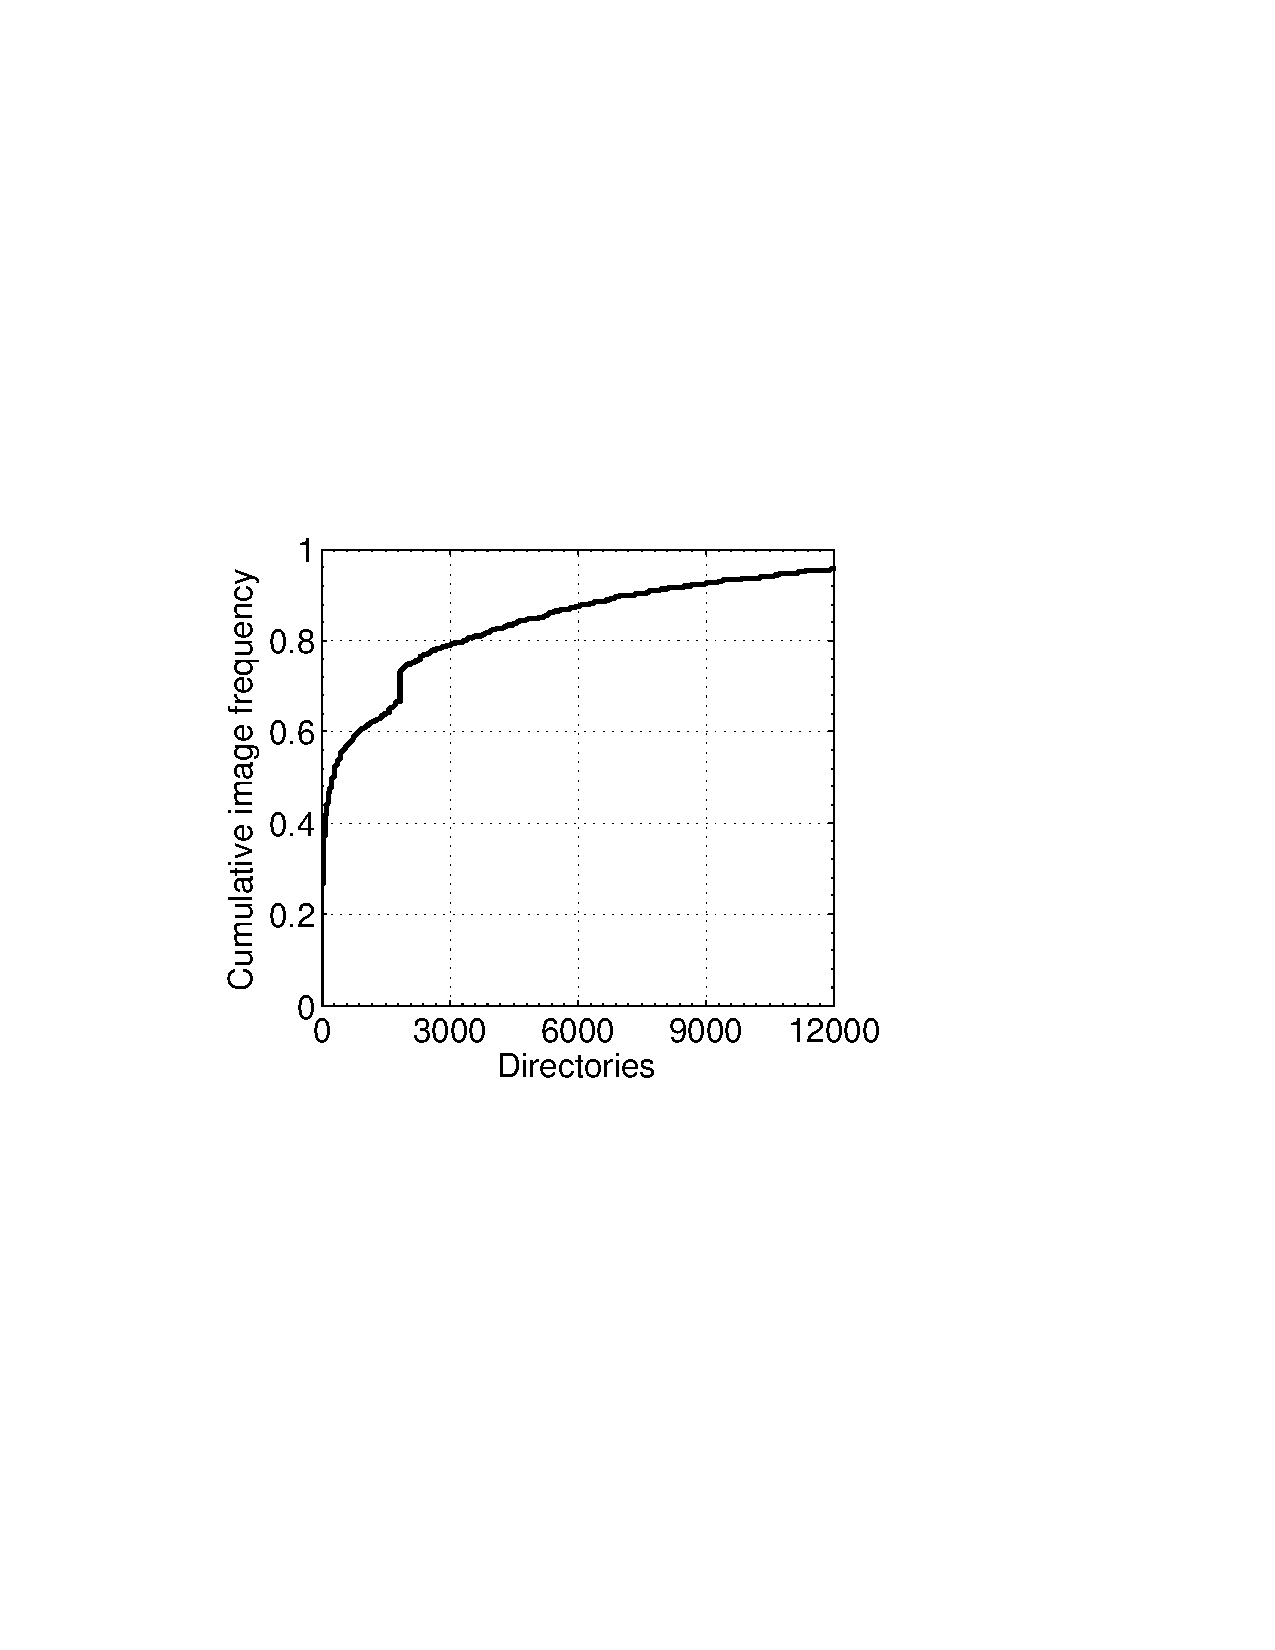
\includegraphics[width=1\textwidth]{graphs/dir.pdf}
%		\caption{CDF of images by\newline directories}
%		\label{fig-dir}
%	\end{minipage}%
%	\begin{minipage}{0.24\textwidth}
%		\centering
%		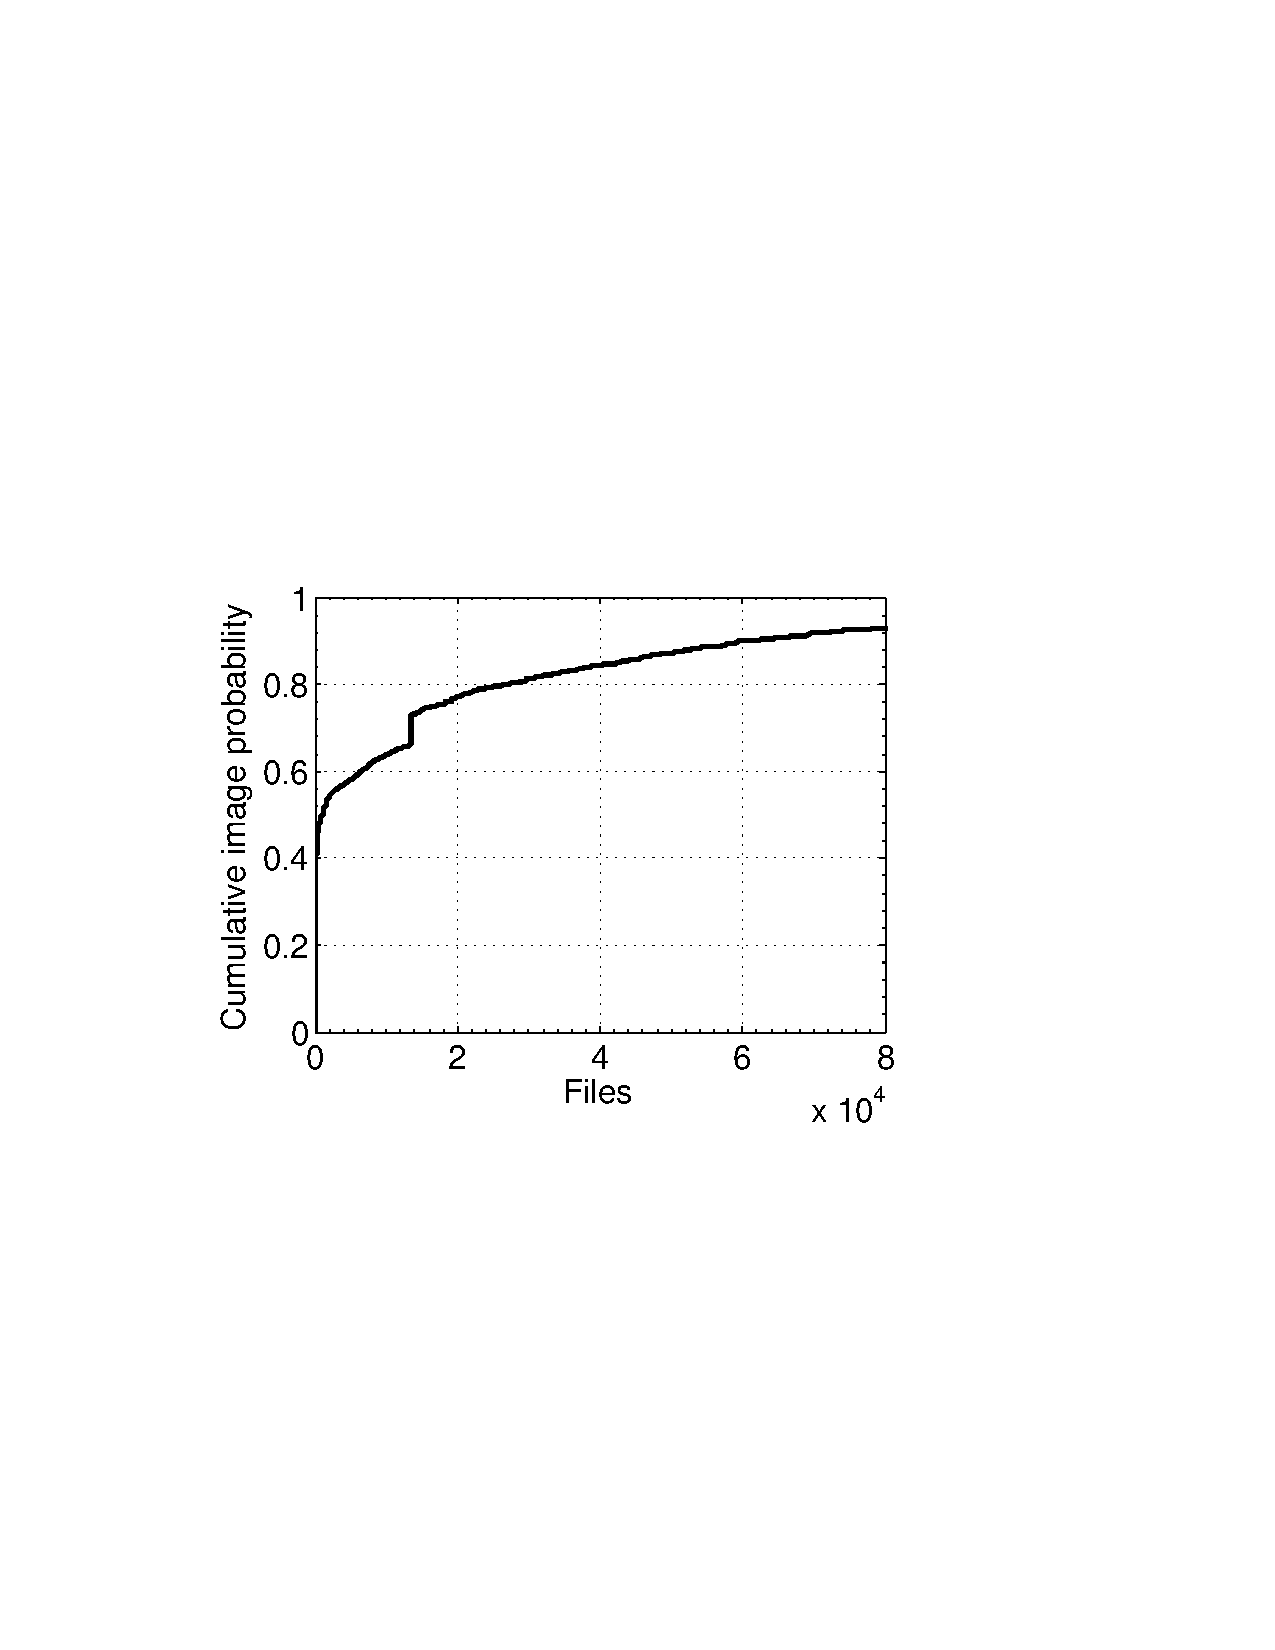
\includegraphics[width=1\textwidth]{graphs/file.pdf}
%		\caption{CDF of images by files}
%		\label{fig-file}
%	\end{minipage}
%\end{figure}

%\begin{figure}[htbp] 
%	\begin{minipage}{0.5\linewidth} 
%		\centering 
%		\includegraphics{circle} 
%		\caption{A Circle} 
%		\label{fig:circle} 
%	\end{minipage}% 
%	\begin{minipage}{0.5\linewidth} 
%		\centering 
%		\includegraphics{rectangle} 
%		\caption{A Rectangle} 
%		\label{fig:rectangle} 
%	\end{minipage} 
%\end{figure}

%
To overcome the deduplication overhead, we analyze registry workloads
and optimize the performance by exploring workload patterns and user
access patterns.
%
We observe that when a Docker client \texttt{pulls} an image
from Docker registry, it will first \texttt{GET} the manifest of the
image, which is metadata file of the image and contains a list of layers'
digests.
%
After that, the client parses the manifest, to find the list of layers
referenced by the image, and compares against a \emph{local layer index}.
%
If a layer doesn't exist in the local layer index, the client will \texttt{GET}
this layer.
%
Thus, we can maintain a \emph{user local layer index} on registry side to keep
track of user access history and predict which layer will be requested by the
user when the user issues a \texttt{GET} manifest request.
%
Typically, if a layer is already stored locally, then the client will not
\texttt{GET} this layer again.
%
However, for Kubernetes, users can configure different policies, such as
\emph{IfNotPresent (i.e, GET if not present)} or \emph{Always GET}.
%
\cite{dockerworkload} presents IBM cloud registry workload traces spanning
$\sim$80 days for 7 different registry clusters: \texttt{Syd}, \texttt{Dal},
\texttt{Fra}, \texttt{Lon}, \texttt{Dev}, \texttt{Pre}, and \texttt{Sta}.
%
%
Figure~\ref{fig:layer-repull-cdf} shows the
CDF of layer \texttt{GET} count by the same clients. 
%
Majority of layers are only fetched once by the same clients.
For example, 97\% of layers from \texttt{Syd} are only fetched once by the same
clients.
%
We also observe that few clients \emph{GET} the same layers continuously.  For
example, a client from \texttt{Lon} fetched the same layer 19,300 times.
%When different clients \texttt{pull} the same repository, they will fetch
%different amount of layers from the repository based on the contents of their
%local layer dataset.  The local layers can vary with time due to clearing of
%the data so the same clients can fetch different amounts of layers at
%different times.  Therefore, a \texttt{pull manifest} request doesn't usually
%result in repulling all the layers in the repository.  Here, we define
%\emph{repulling a repository} as repulling the layers in the repository for
%the same client.  Figure~\ref{fig:repo-repull-cdf} shows the CDF of the
%probability of repository repulling, calculated as the number of \texttt{pull
%manifest} resulting in repository repulling divided by the total number of
%\texttt{pull manifest} requests issued for the same repository.  We see that
%majority of repositories aren't repulled.  The percentage of repositories
%whose repull probability is zero (i.e. are pulled only once by a client)
%ranges from 57\% for \texttt{Prestage} to 85\% for \texttt{Syd}.  Only 20\% of
%repositories from  \texttt{Prestage}, \texttt{Stage}, and \texttt{Syd} have a
%repulling probability higher than 0.5.  We also observe that few repositories'
%repulling probability is 1, indicating repulls everytime by the clients.

We define \emph{repulling} as the act of fetching the same layer more than once
by the same user.
% before because they are no longer present on the user side.
Figure~\ref{fig:client-repull-cdf} shows the client repulling probability,
calculated as the number of \emph{repulling} layer requests divided by the
number of total \texttt{GET} layer requests issued by the same client.
%
We see that a significant amount of clients have a low repulling proability.
%
For example, 71\% of clients from \texttt{syd} have a repulling probability lower
than 0.1.
%
Very few clients have a high repulling probability.  For instance,
only 2\% clients have a repulling probability higher than 0.9 from
\texttt{Dal}.


We also observe that the slope is steep at both lower and higher probabilities.
However, the slope becomes flat in the middle.
%
For example, the slope at probabilities between 0.1 and 0.9 for \texttt{dev}
almost equals to zero.
%
In this case, the high repulling probability clients can be classified as
always-pull clients, and the low repulling probability clients as pull-once
clients.
%
The few clients in the middle are considered as \emph{erratic}.
%
Thus, to determine whether a client will \texttt{repull} a layer or not, we
consider the client repulling probability and the layer repull count.
%From the probability distribution of the clients repulling, we can observe
%that a significant chunk of the clients have very low repulling probability
%and another chunk of the clients have a very high repulling probability, with
%few clients in the middle. For simplicity of implementation, the high
%probability clients can be classified as always repulling clients, and the low
%probability clients as never repulling (i.e. they pull only once). The few
%clients in the middle are considered as \emph{erratic} and no classification
%is made for them.



\subsection{Layer preconstruction}
%\begin{figure*}[t]
%		\begin{minipage}{0.32\linewidth}
%			\centering
%			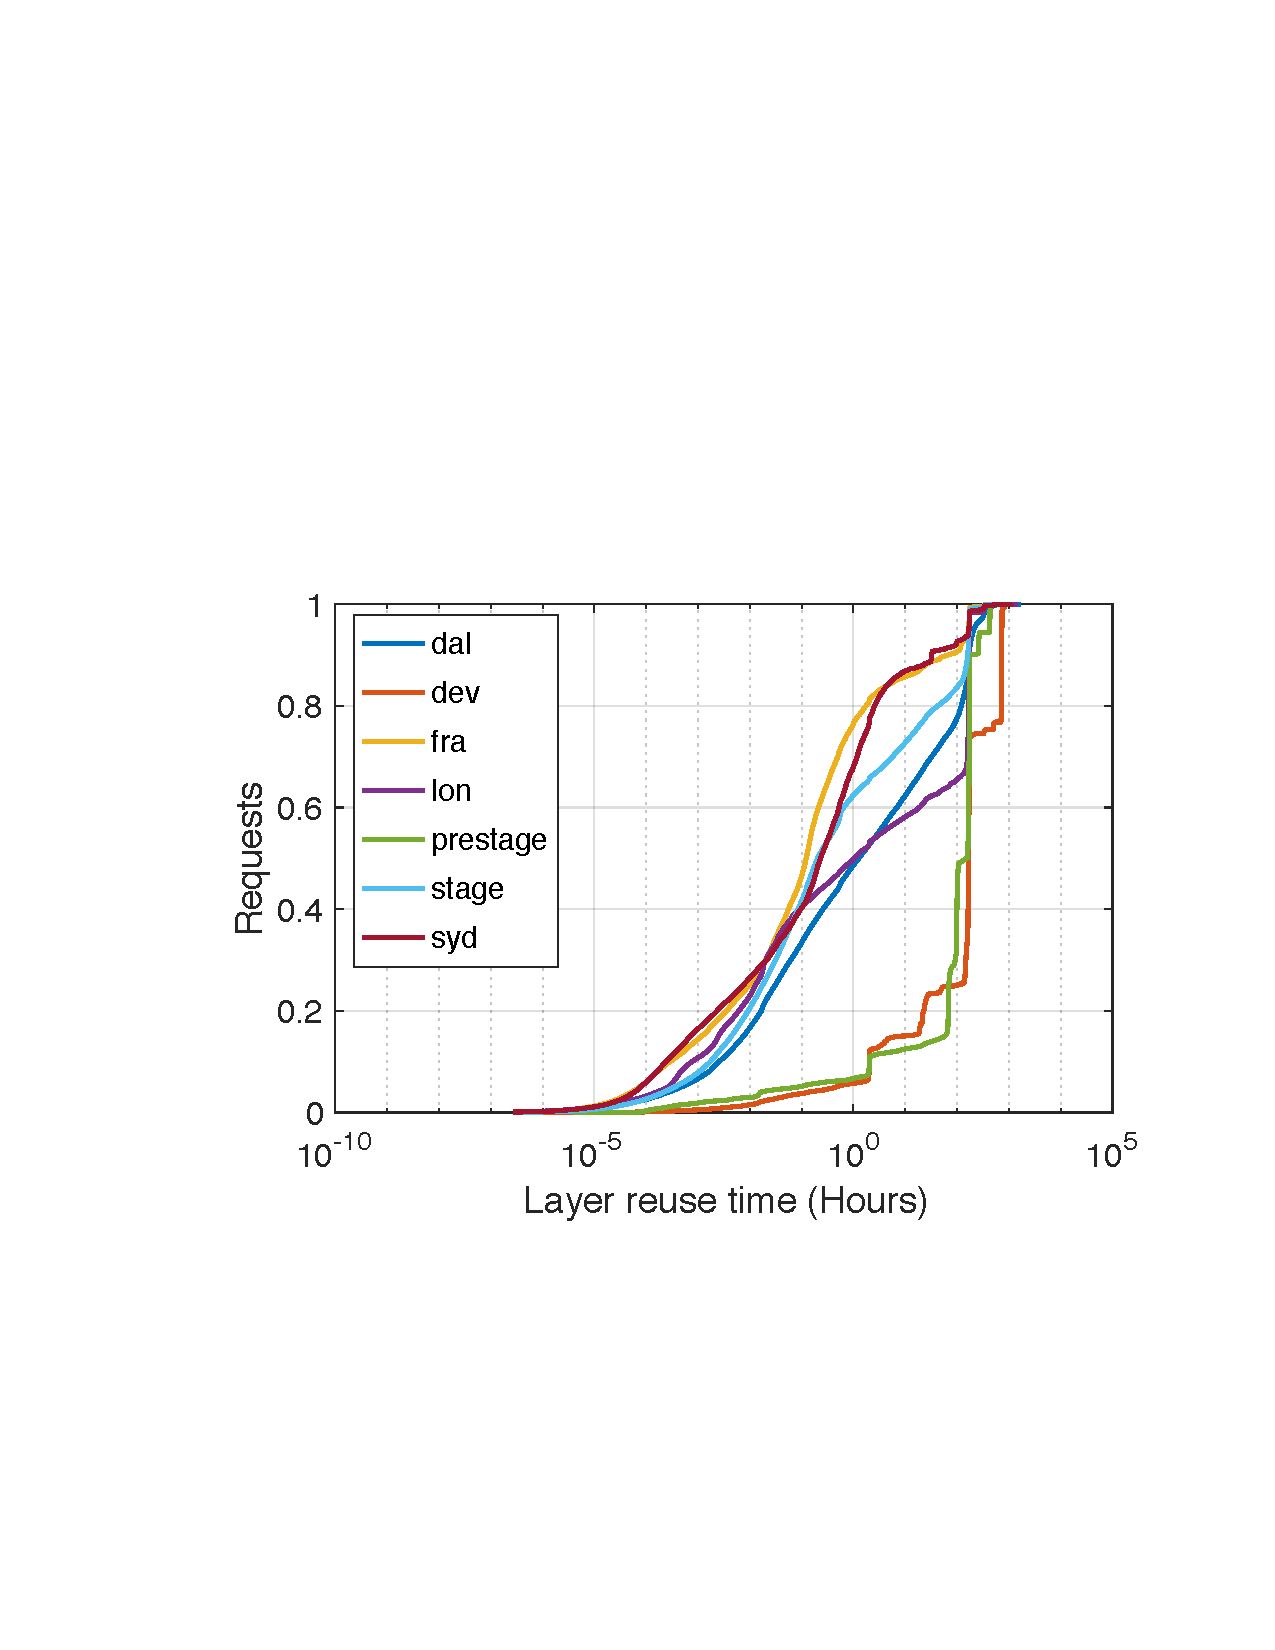
\includegraphics[width=1\textwidth]{graphs/layer-reusetime.pdf}
%		%	\caption{CDF of layer reuse time.}
%		%	\vspace{-3pt}
%			\label{fig:layer-reuse}
%		\end{minipage}
%			\begin{minipage}{0.32\linewidth}
%				\centering
%				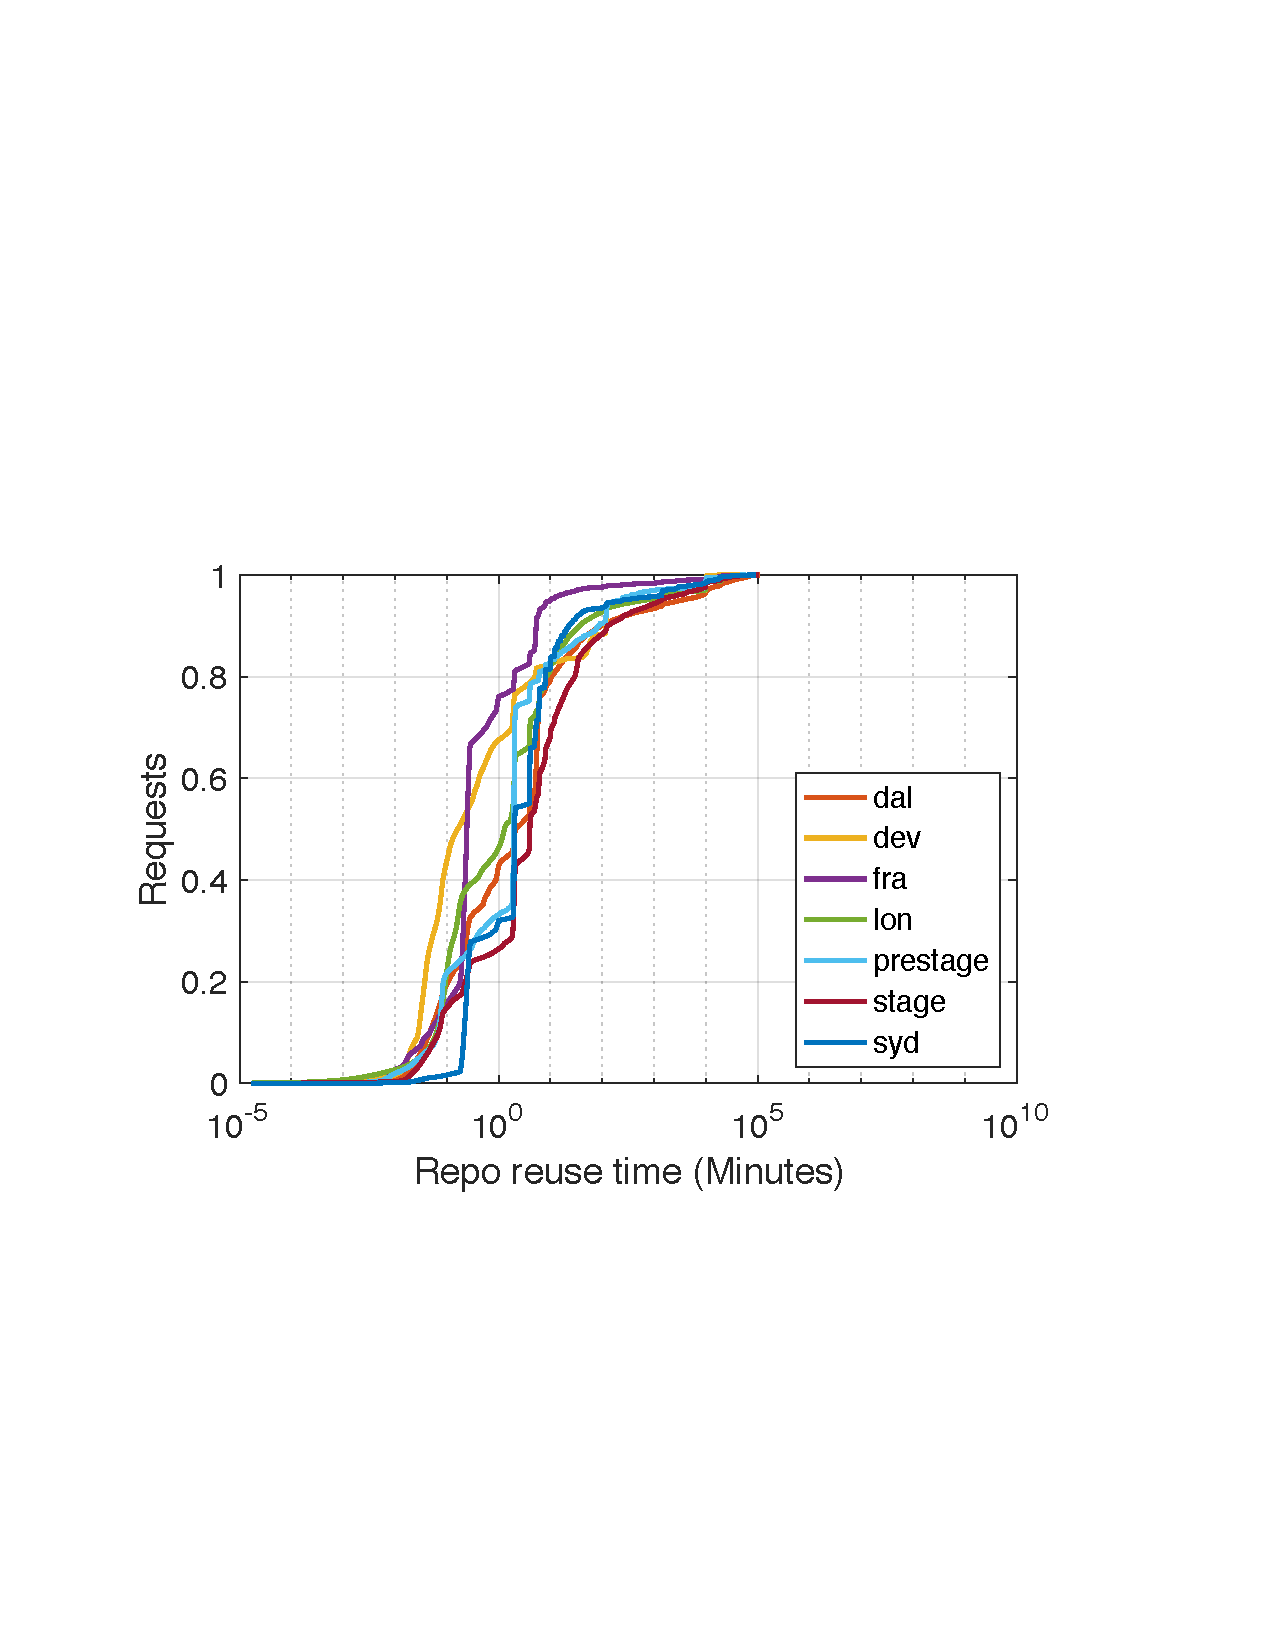
\includegraphics[width=1\textwidth]{graphs/repo-reusetime.pdf}
%			%	\caption{PDF of repository reuse time.}
%				%	\vspace{-3pt}
%				\label{fig:repo-reuse}
%			\end{minipage}
%		\begin{minipage}{0.32\linewidth}
%			\centering
%			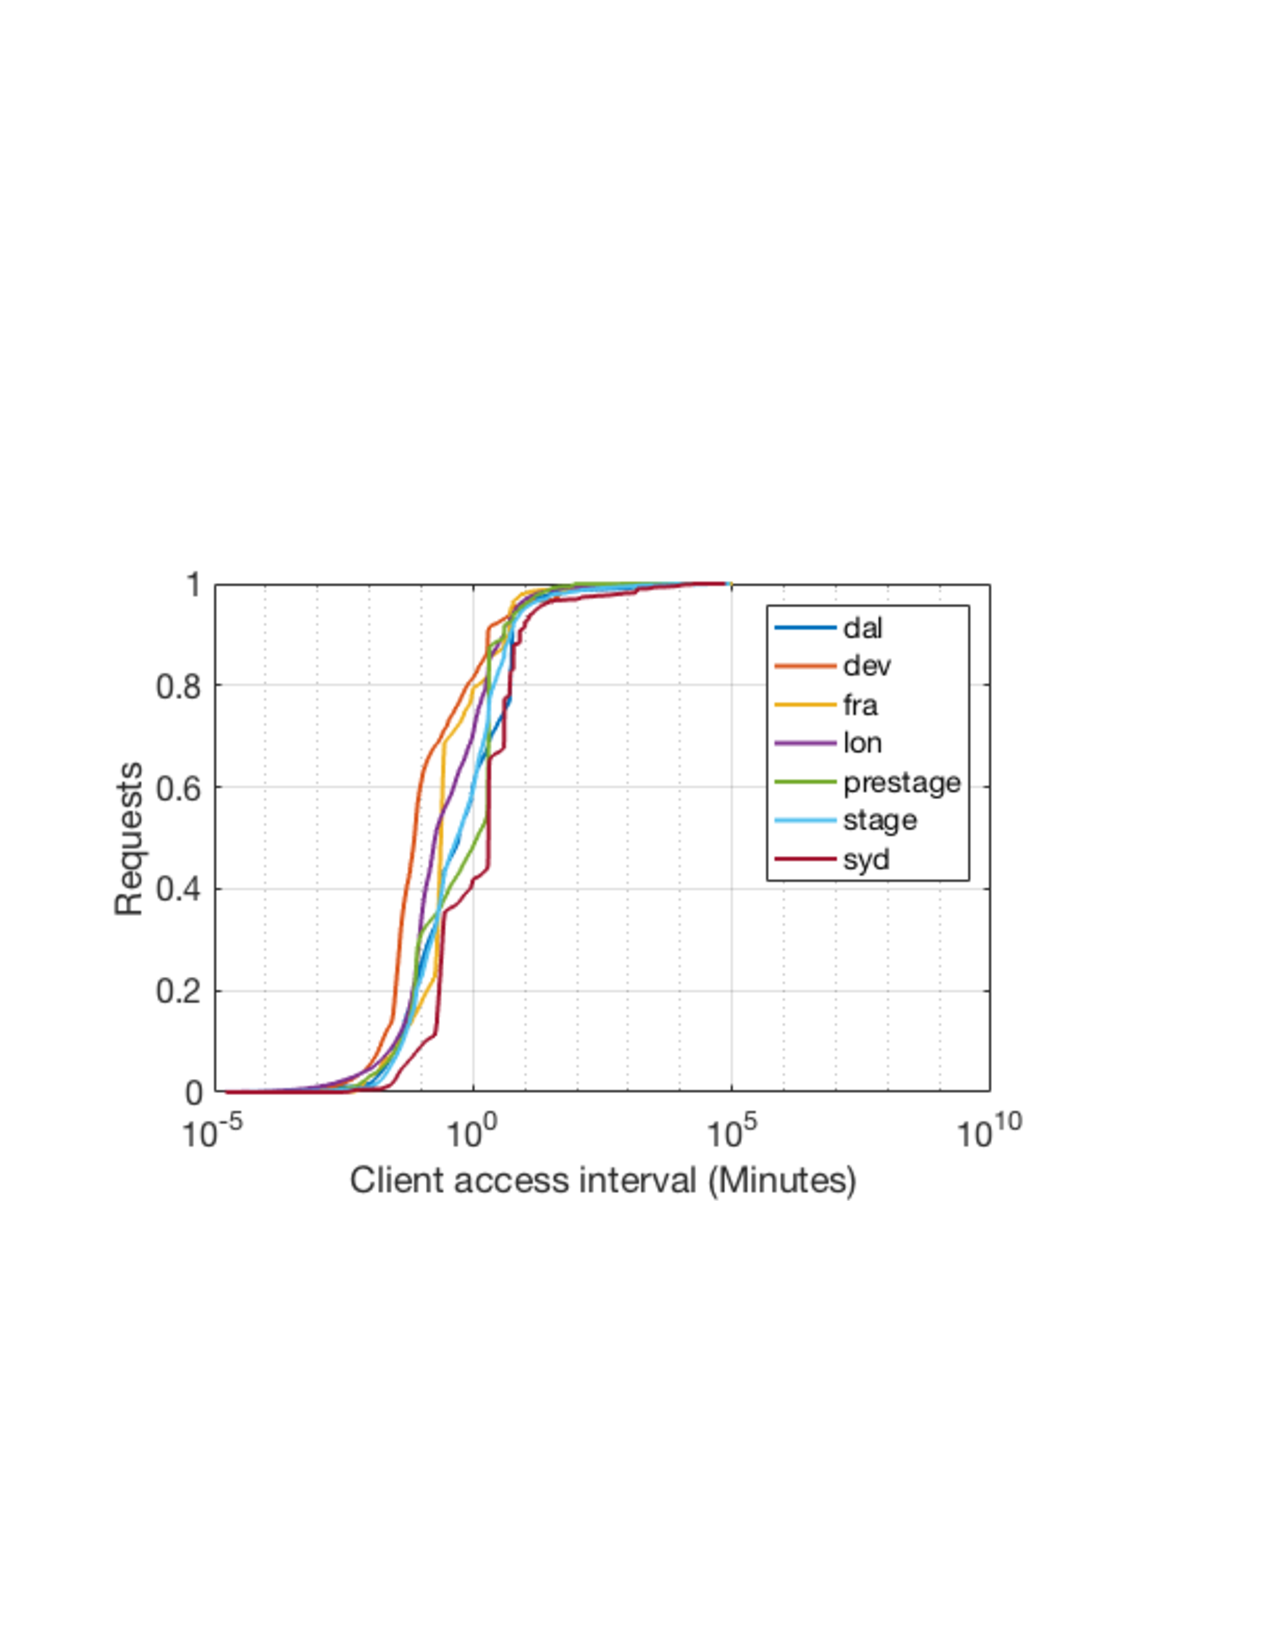
\includegraphics[width=1\textwidth]{graphs/user-intervals.pdf}
%			%\caption{PDF of client access intervals.}
%			%	\vspace{-3pt}
%			\label{fig:user-interval}
%		\end{minipage}
%	\caption{CDF of reusetime for layers, repositories and clients' access intervals.}
%	\label{fig:layer-reuse}
%\end{figure*}
\begin{figure}[t]
	\centering
	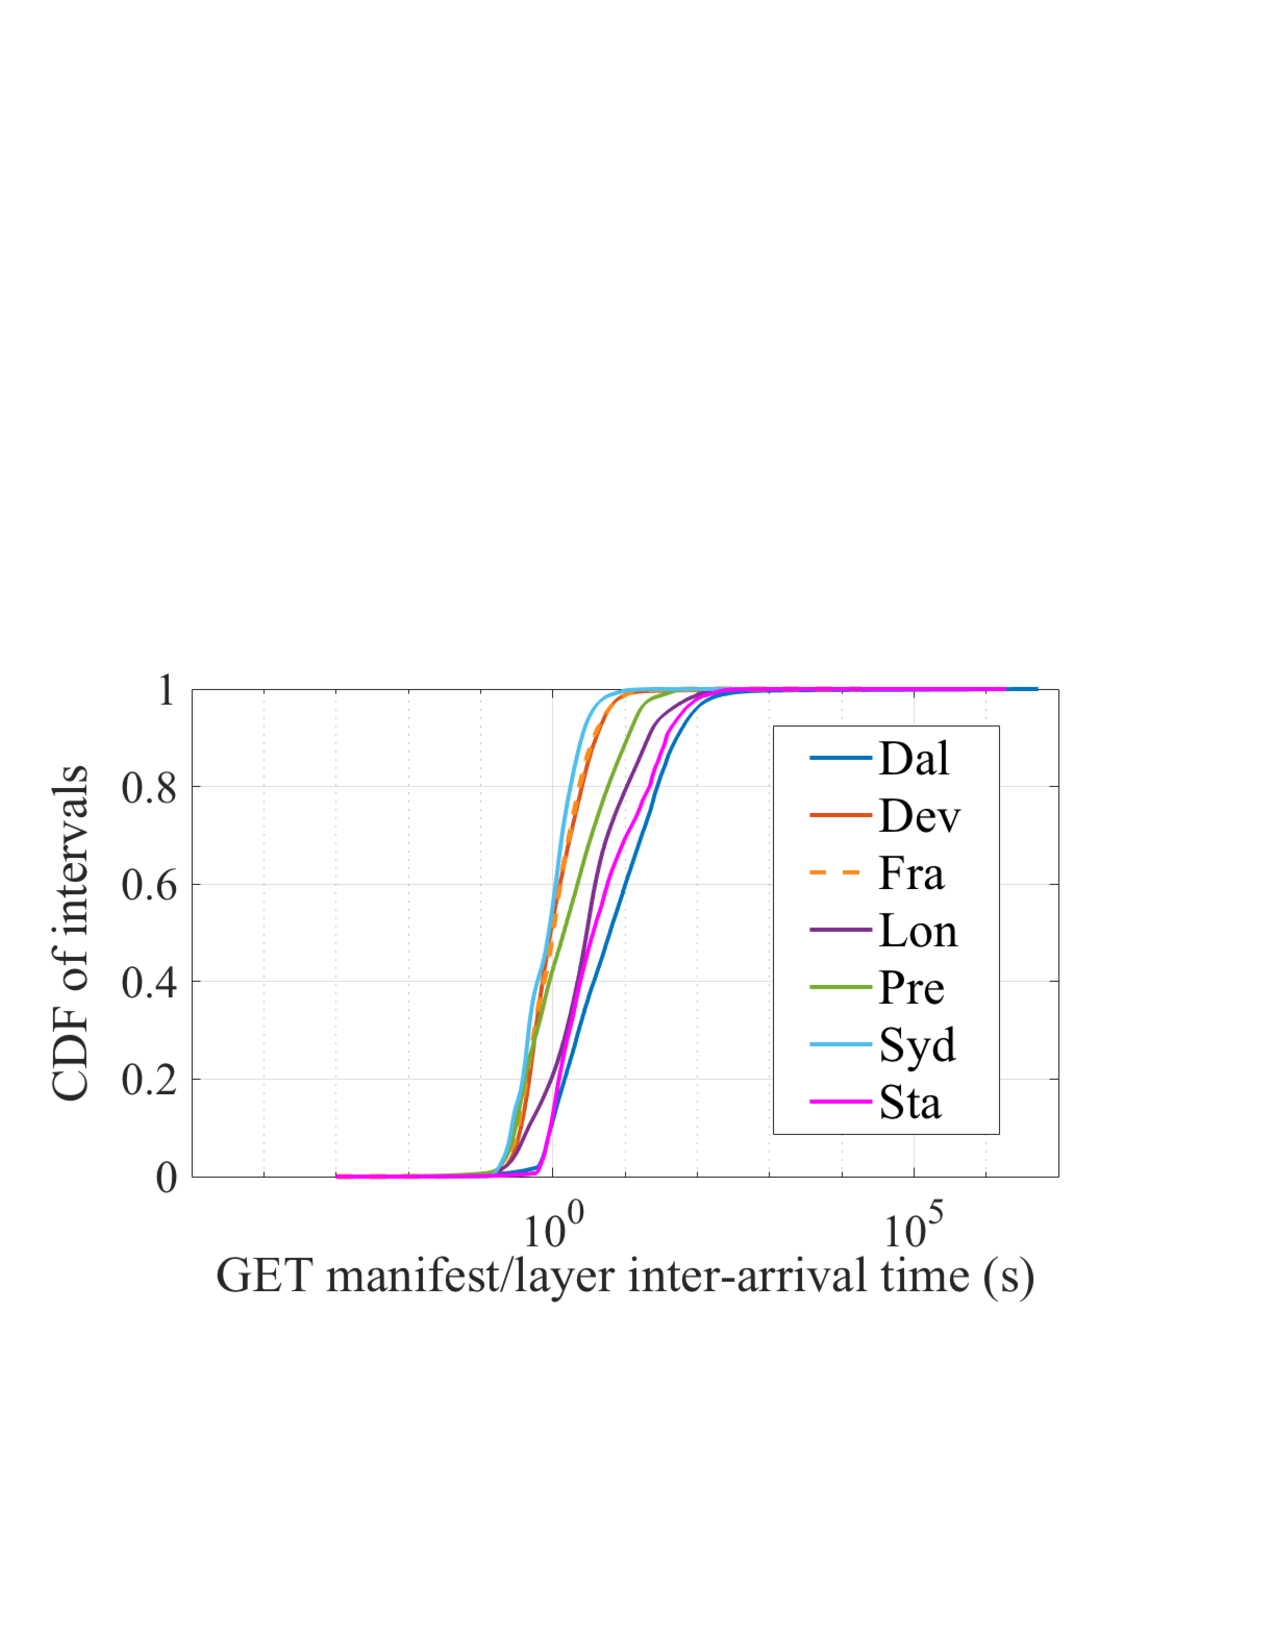
\includegraphics[width=0.3\textwidth]{graphs/GML-intervals.pdf}
	\caption{Intervals between \texttt{pull} manifest request and \texttt{pull} layer request}
	%	\vspace{-3pt}
	\label{fig:intervals}
	
\end{figure}
%\begin{figure*}[!t]
%	\centering
%	\subfigure[Layer repull count]{
%		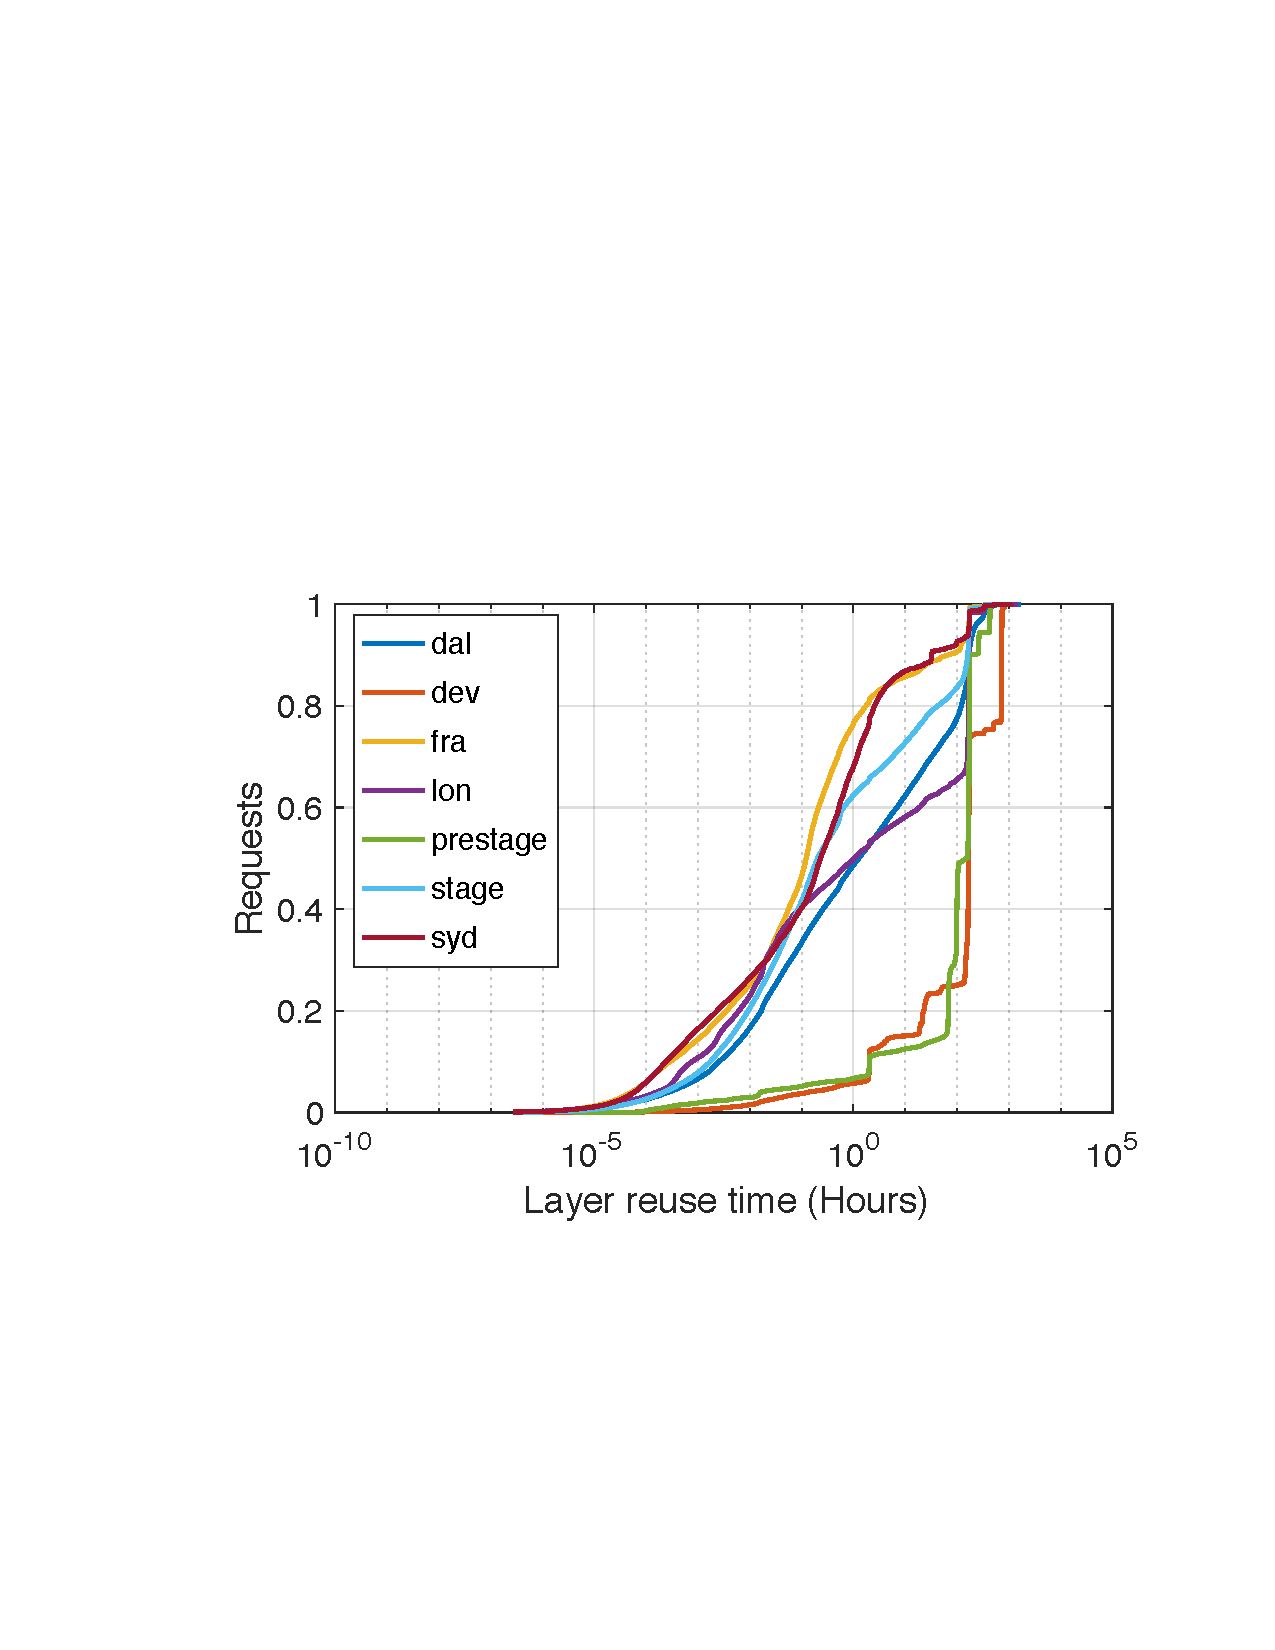
\includegraphics[width=0.2\linewidth]{graphs/layer-reusetime.pdf}
%			\label{fig:layer-reuse}
%	}
%	\subfigure[Repository repulling probability]{
%		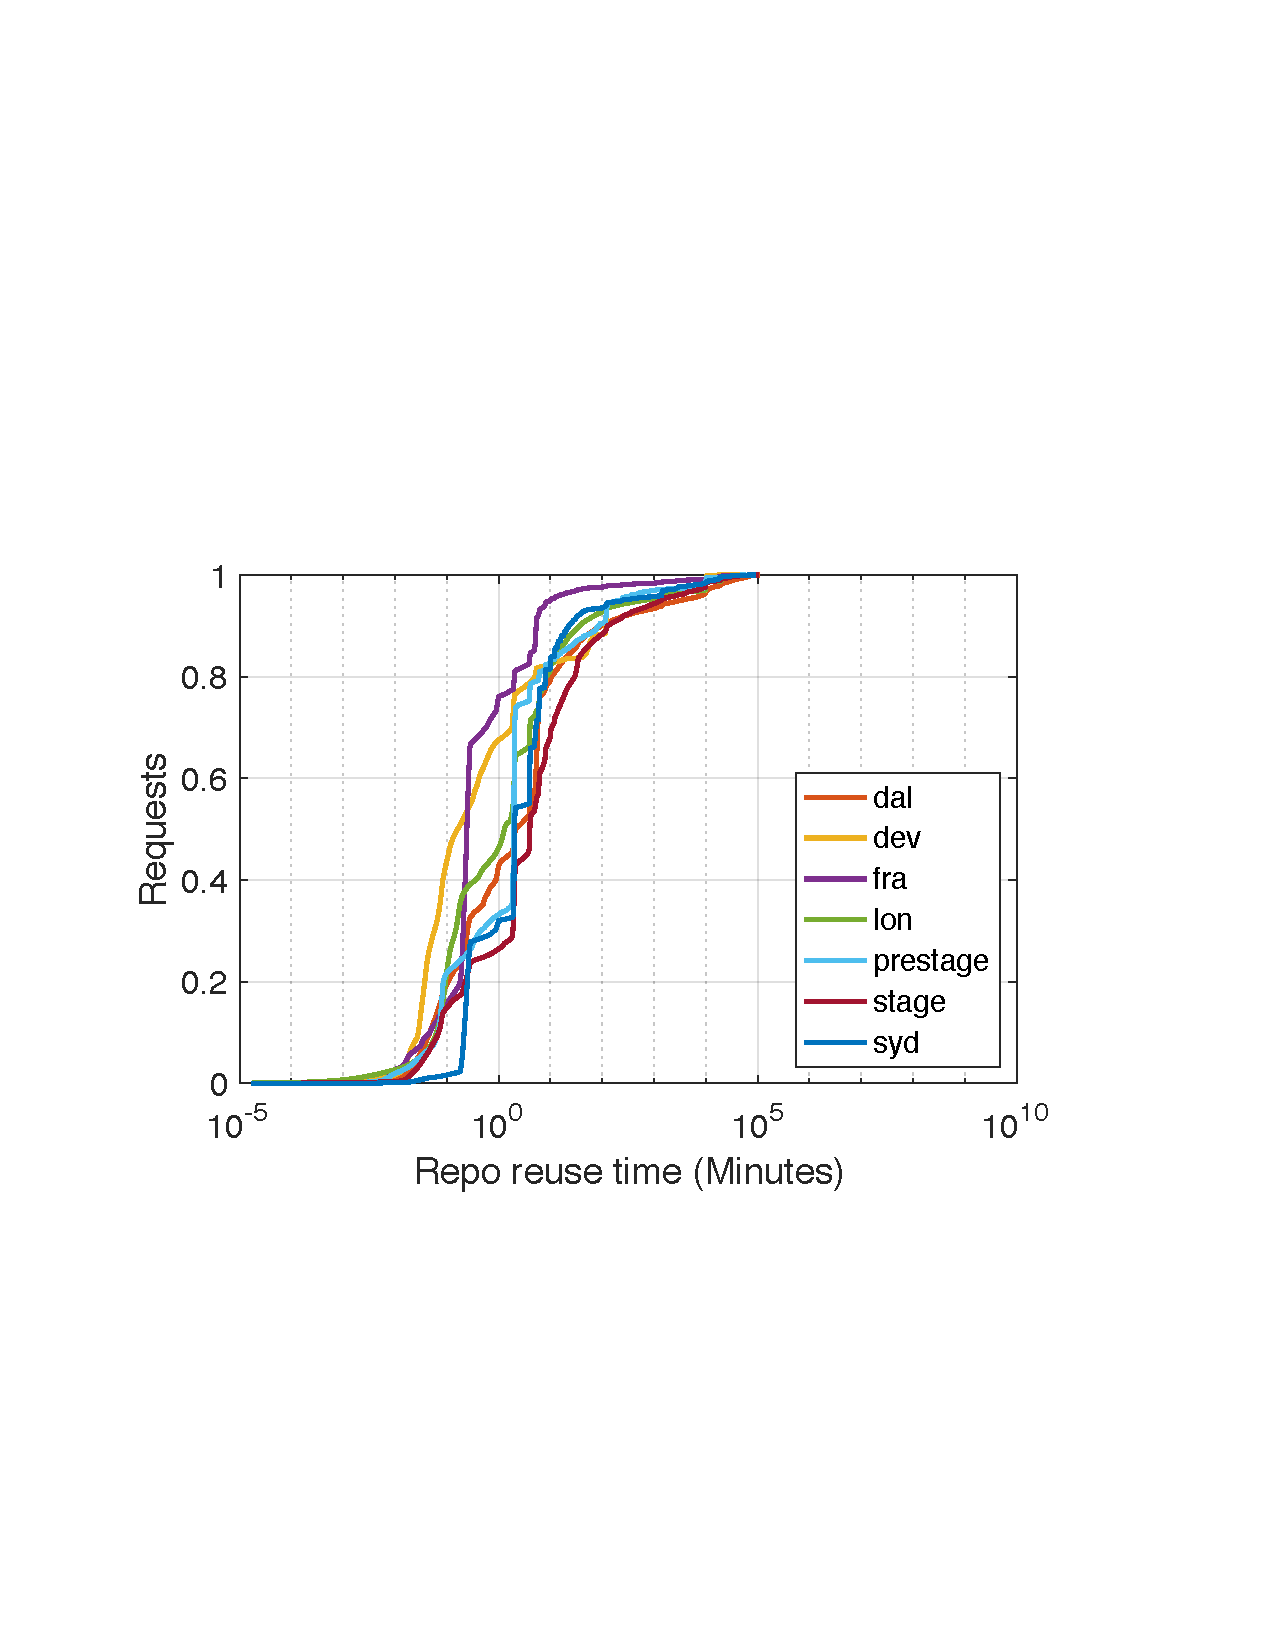
\includegraphics[width=0.2\linewidth]{graphs/repo-reusetime.pdf}
%				\label{fig:repo-reuse}
%	}
%	\subfigure[Client repulling probability]{
%		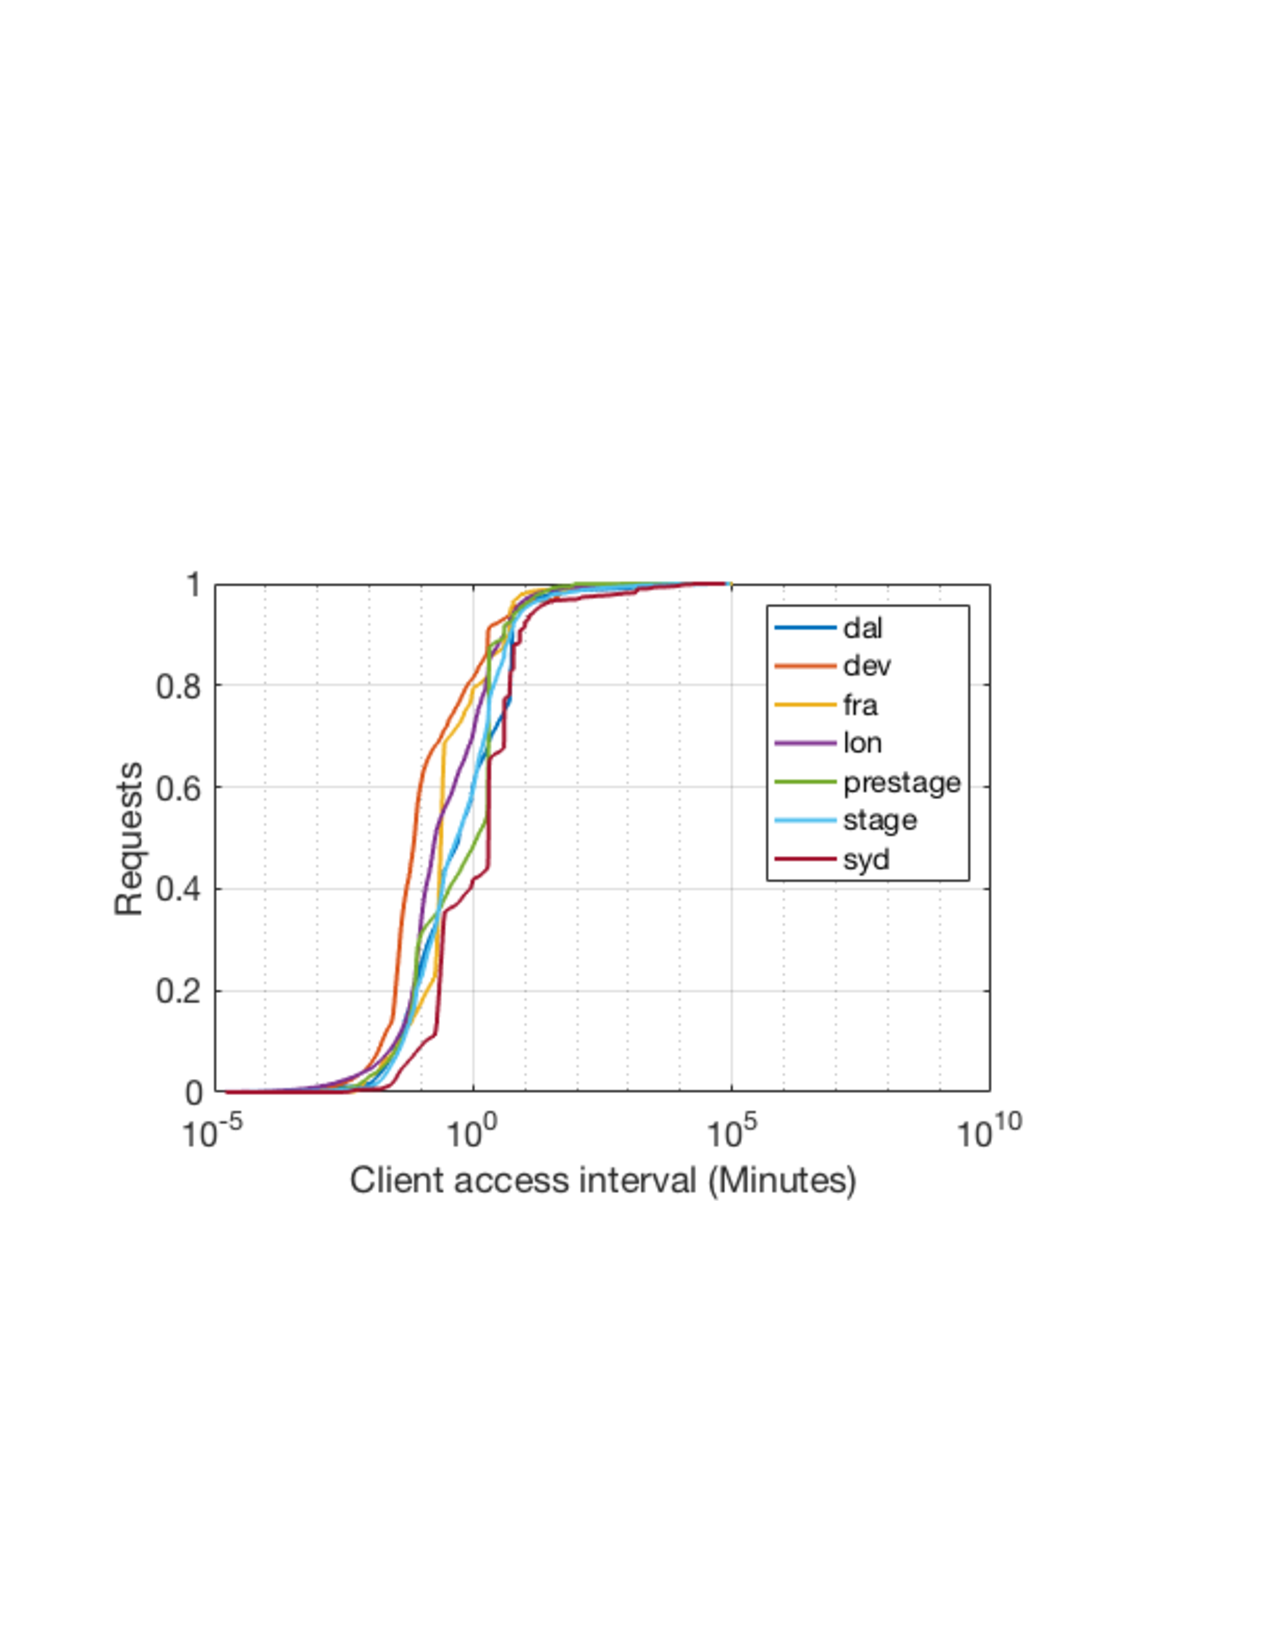
\includegraphics[width=0.2\linewidth]{graphs/user-intervals.pdf}
%			\label{fig:user-interval}
%	}
%	\caption{CDF of reusetime for layers, repositories and clients' access intervals.}
%	\label{fig:fig-reuse}
%\end{figure*}

%\begin{figure}[t]
%	\centering
%	\begin{minipage}{0.26\textwidth}
%		\centering
%		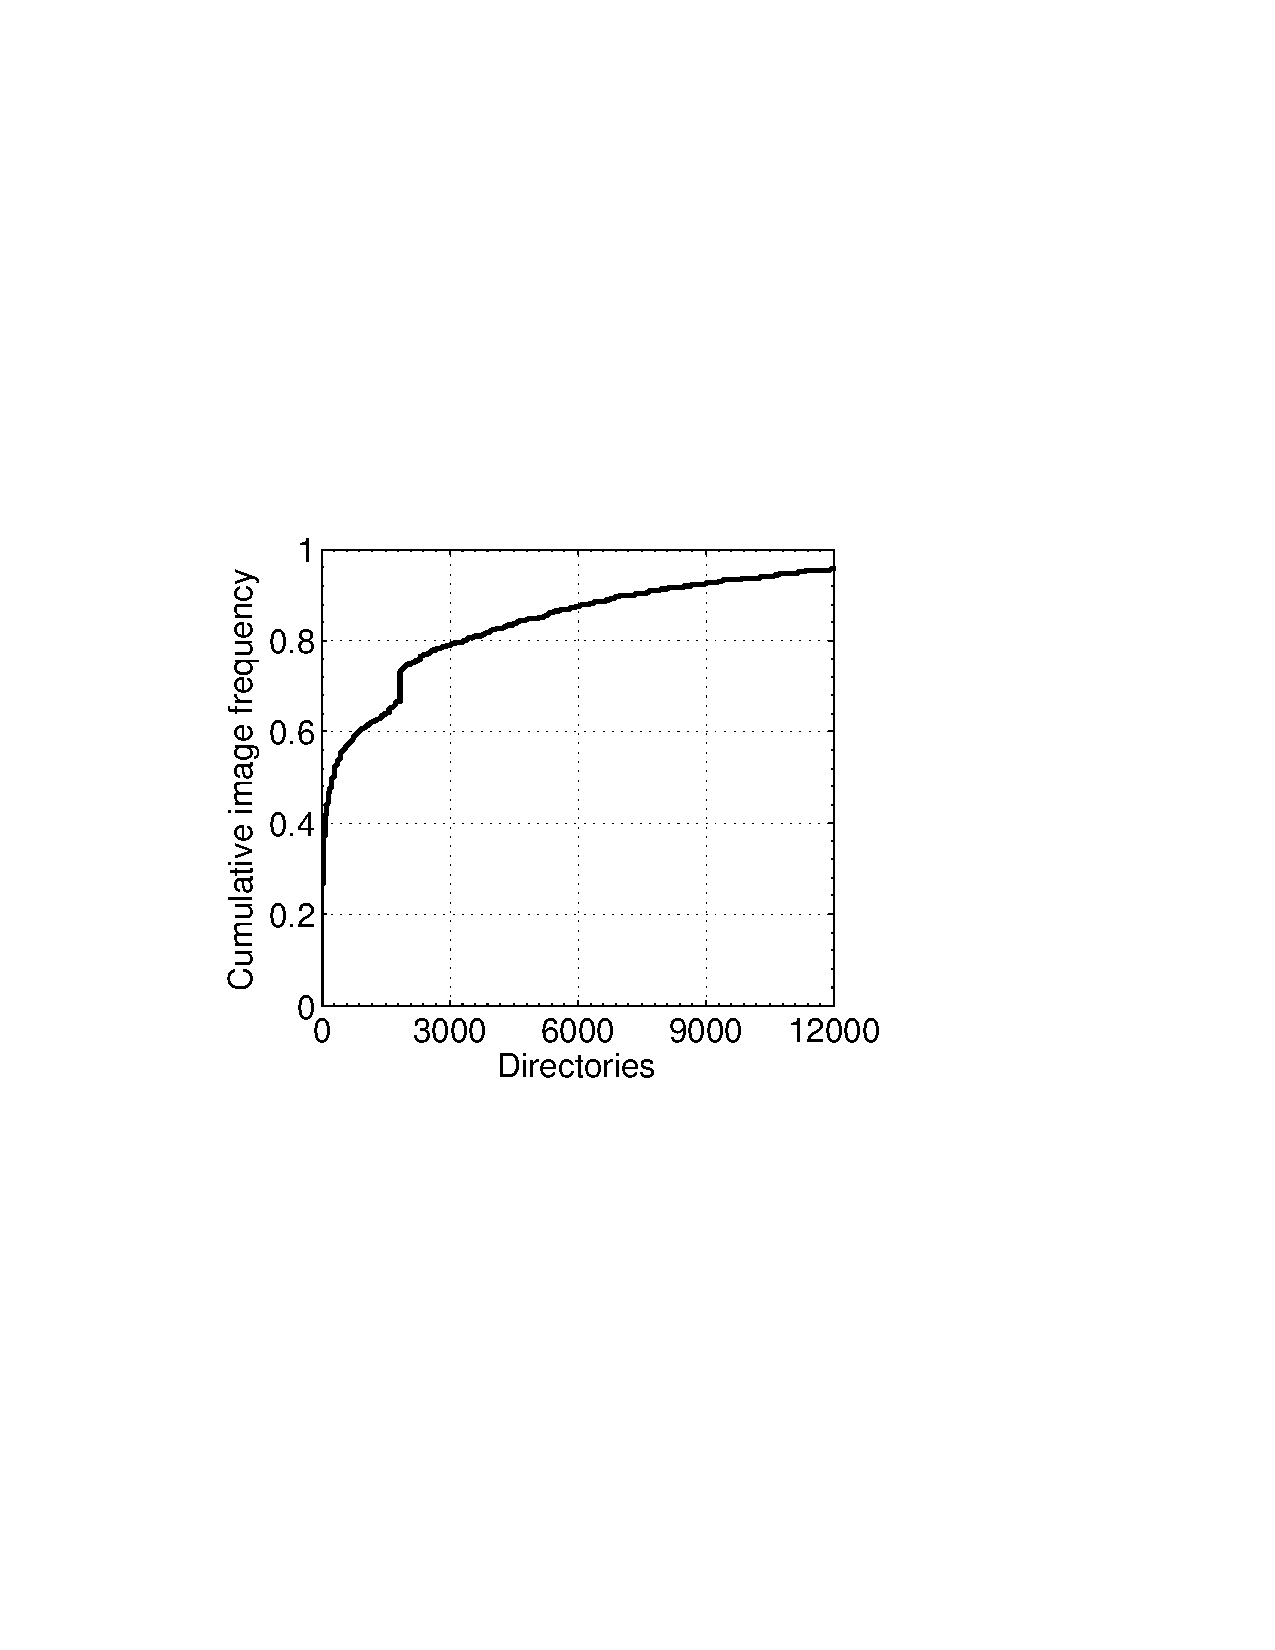
\includegraphics[width=1\textwidth]{graphs/dir.pdf}
%		\caption{CDF of images by\newline directories}
%		\label{fig-dir}
%	\end{minipage}%
%	\begin{minipage}{0.24\textwidth}
%		\centering
%		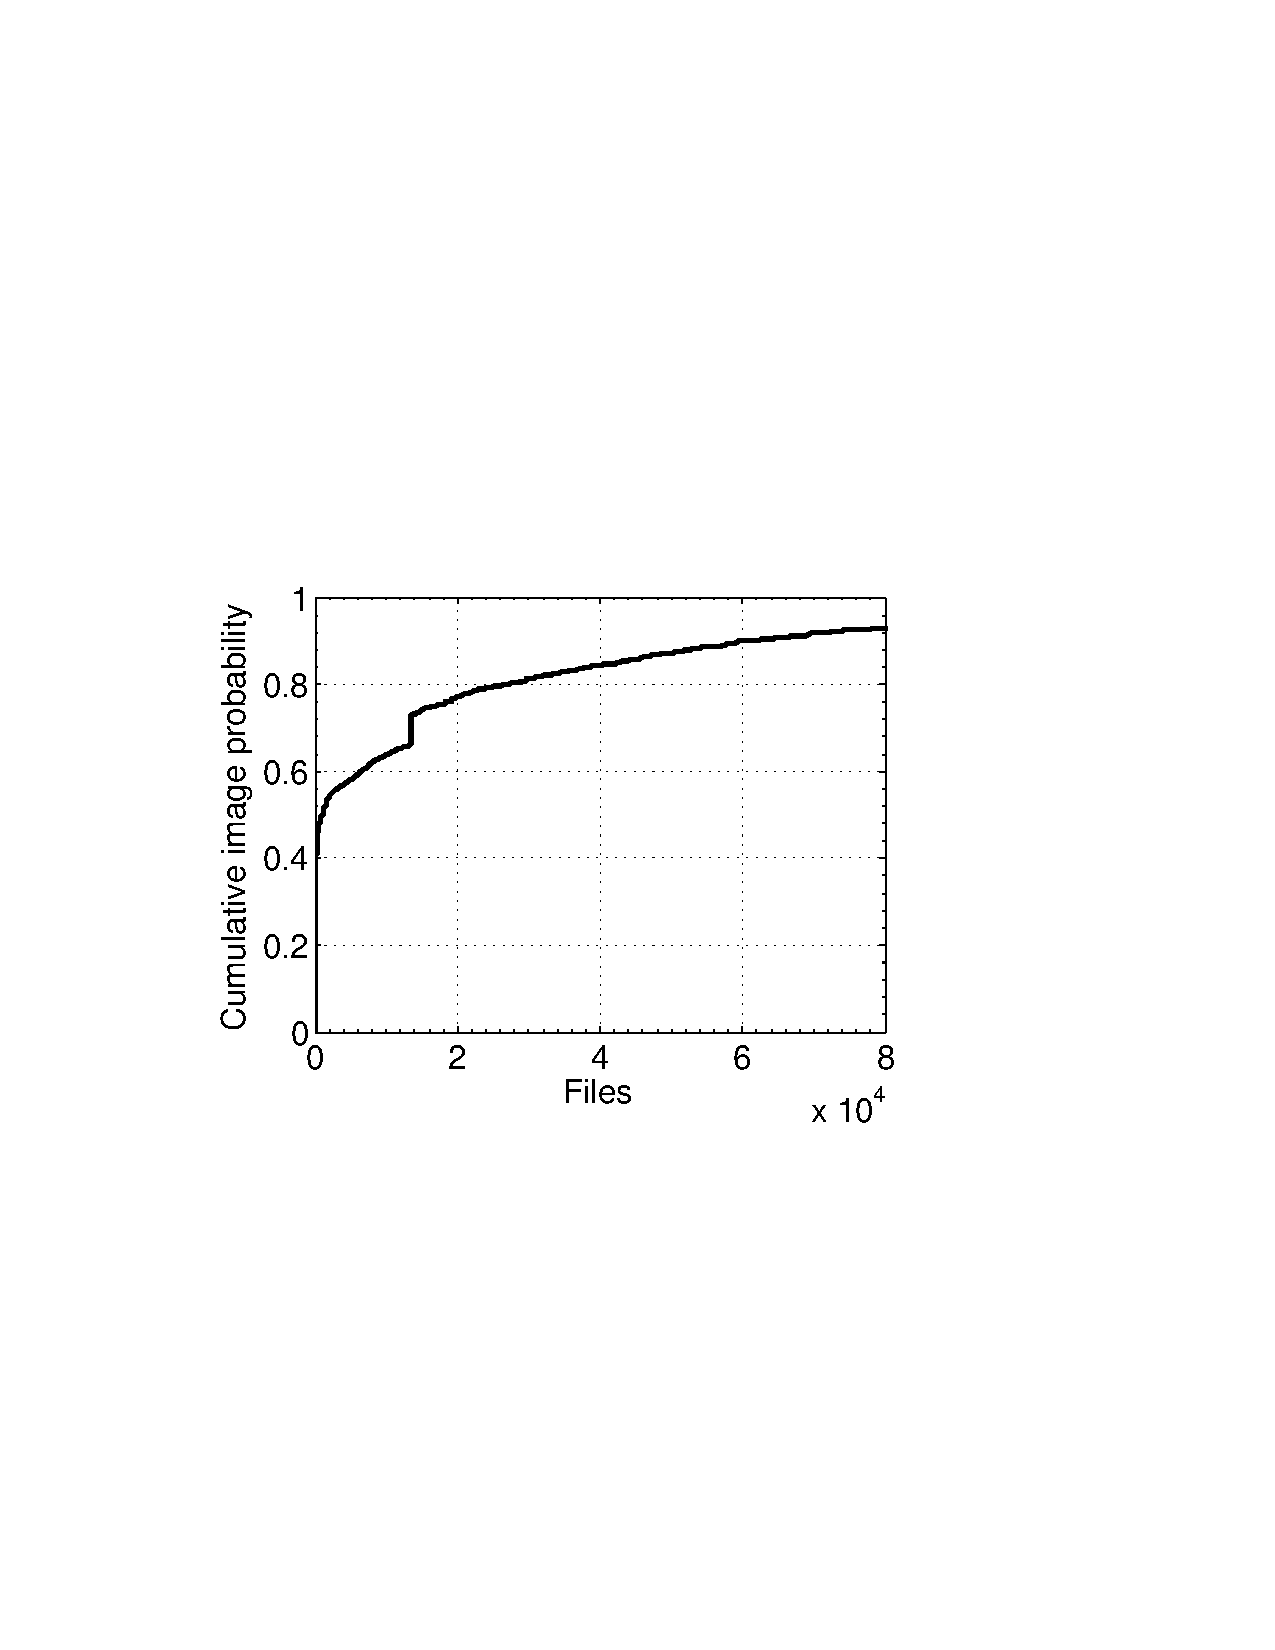
\includegraphics[width=1\textwidth]{graphs/file.pdf}
%		\caption{CDF of images by files}
%		\label{fig-file}
%	\end{minipage}
%\end{figure}

%\begin{figure}[htbp] 
%	\begin{minipage}{0.5\linewidth} 
%		\centering 
%		\includegraphics{circle} 
%		\caption{A Circle} 
%		\label{fig:circle} 
%	\end{minipage}% 
%	\begin{minipage}{0.5\linewidth} 
%		\centering 
%		\includegraphics{rectangle} 
%		\caption{A Rectangle} 
%		\label{fig:rectangle} 
%	\end{minipage} 
%\end{figure}
%
%As shown in~\cite{xxx}, layer accesses are heavy skewed.  There are hot layers
%that account for majority of layer accesses.  Hence, we can cache hot layers
%to improve performance.
As another optimization we explore if it is possible to preconstruct a 
deduplicated layer before users iisues a \texttt{GET} layer to avoid the
the time spend in layer restoration.
%
We analyze the duration between a \texttt{GET} manifest request and the subsequent
\texttt{GET} layer request and show in Figure~\ref{fig:intervals}.
%
We observe that majority of intervals are greater than one second.
%
For example, 80\% of intervals from \texttt{lon} are greater than one second.
%
Whereas, 60\% of the intervals from \texttt{syd} are greater than five seconds. 
%
Hence, there is a relatively long gap
between a \texttt{GET} manifest request and the subsequent \texttt{GET}
layer requests.
%
This is because, first, when fetching an image from a registry,
Docker client \emph{downloads} a certain number layers in parallel (three by
default) starting from the lowest or base layers.
%
In a case where an image
contains more than three layers, then the \emph{upper} layers have to wait untill the
\emph{lower} layers are downloaded, which varies the \texttt{GET} layer request
arrival time for the registry.
%
Second, network delay between clients and registry
often accounts for a greater proportion of the \textt{GET} layer latency in Cloud
environment, especially for the large layers.
%
Consequently, we can use this long
gap to predict which layers will be fetched by the user when a \texttt{GET}
manifest request is received, and then build a layer for the user before
the \texttt{GET} layer request arrive.


